%\documentclass[12pt]{article}
%\usepackage{amsmath}
%\usepackage{graphicx, color}
%\usepackage{amssymb}
%\usepackage{listings} %source code listing
%\usepackage{multirow}
%%\usepackage[version=2]{mhchem}
%\usepackage{subfig}
%\usepackage{hyperref}
%\usepackage{units}
%\usepackage{gensymb}
%\usepackage{adjustbox}
%\usepackage{listings}
%\usepackage{color}
%\usepackage{tcolorbox}
% 
%\definecolor{codegreen}{rgb}{0,0.6,0}
%\definecolor{codegray}{rgb}{0.5,0.5,0.5}
%\definecolor{codepurple}{rgb}{0.58,0,0.82}
%\definecolor{backcolour}{rgb}{0.95,0.95,0.92}
%
%\newcommand{\specialcell}[2][c]{%
%  \begin{tabular}[#1]{@{}c@{}}#2\end{tabular}}
% 
%
%
%\title{Reactor physics with Python \\ Lecture Notes}
%
%
%\author{Zs.~Elter. E. Branger, M. Preston \\ Uppsala University \\
%        Division of Applied Nuclear Physics}%\corref{cja}}
%%
%\date{2021.}
%\begin{document}

\section{Neutron transport and diffusion}

In this section we are going to derive an equation describing neutron transport in general. This equation is the basis of reactor physics, and can be approximated in several ways to study only certain parts of neutron physics.

Several course books introduces neutron transport immediately by jumping into neutron diffusion and considering that neutrons move around in materials or in a reactor as gas molecules would. In this case one assumes that neutrons tend to diffuse from regions of high neutron density to regions of low neutron density (which is qualitatively usually true, but the quantitative relation ship between flux and current density is where the approximation comes in). One reason for this approach is that solving the neutron transport equation is intimidating, or in most realistic cases it is even impossible, whereas handling the diffusion formalism is more straightforward.

However, deriving the exact neutron transport equation is actually simpler than deriving the diffusion equation, and since it describes reality better, it is actually worth to start from here, and later turn our attention towards diffusion which is an approximations of neutron transport theory. Therefore after deriving the general transport equation we will simplify it to reach the diffusion theory, which we will use to have a basic understanding of the spatial distribution of neutrons in a reactor core.

The main goal of neutron transport, and thus this chapter is to tracking the population of neutrons at any point of the reactor, thus determine the neutron population

\begin{equation}
n(\mathbf{r}, E, \mathbf{\Omega},t) = \:?
\end{equation}

\noindent and to develop a balance equation for the population

\begin{equation}
\frac{\partial n(\mathbf{r}, E, \mathbf{\Omega},t)}{\partial t} = \:? = \text{gains} - \text{losses}
\end{equation}

The main focus of neutron transport is to figure out how to solve for the neutron population density $n(\mathbf{r}, E, \mathbf{\Omega},t)$. If we know this, we will know the location and velocity of all neutrons at all time. To achieve this, we will need to know the reaction rates which can take remove and add neutrons to the system. For all reactions there is an associated change in energy (except forward scattering which is basically a "miss"), change in momentum and direction.

The balance equation is not going to be difficult. We have only couple of reactions which result in "gain" reactions. And when it is about losses, it is really just the total cross section which will come to play, since essentially all reactions result in a loss of a neutron at the certain phase space. Besides this we will have streaming terms: neutrons without reaction might come into our infinitesimal volume and might leave it, and we will be interested in the net outcome of these streaming movements. Nevertheless, as we will soon see, even though the equations developed are rather intuitive and straightforward, their solutions are challenging.

\subsection{Basic quantities: neutron density, flux and current}

In order to describe the population of neutrons in a reactor we will need to introduce several quantities (some of which we have already introduced, although not in their most generic form). In the following we summarize the related chapter of D\&H (p122), and the reader is definitely encouraged to read that for further details.

\begin{figure}[ht!]
\protect \centering{
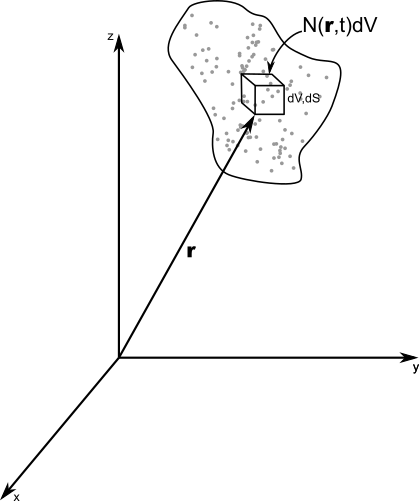
\includegraphics[scale=0.66] {figures/03-neutronpopulation.png}}\protect
\caption{\label{fig:neutronpopulation} \footnotesize{Illustration of neutron population density.}}
\end{figure} 

Let us define the expected number of neutrons in $dr^3$ about $\mathbf{r}$, energy $dE$ about $E$ moving in direction $\mathbf{\Omega}$ in solid angle $d\mathbf{\Omega}$ at time $t$ as the angular neutron population density

\begin{equation}
n(\mathbf{r},E,\mathbf{\Omega},t)dr^3dEd\mathbf{\Omega}
\end{equation}

\noindent Similarly we could define the scalar neutron population density after eliminating certain variables 

$$N(\mathbf{r},t)=\int^\infty_0N(\mathbf{r},E,t)dE=\int^\infty_0\int_{4\pi}n(\mathbf{r},E,\mathbf{\Omega},t)d\mathbf{\Omega}dE$$

\noindent which is illustrated in Figure \ref{fig:neutronpopulation}.

Then we can recall, that the actual physical quantity we can directly measure in a reactor is the reaction rate density (similar reaction rates can be defined for the energy integrated population density, or for the angular density):

\begin{equation}
R(\mathbf{r},E,t)dr^3dE=v(E)\Sigma(E) N(\mathbf{r},E,t)dr^3dE
\end{equation}

\noindent where, due to convenience we usually introduce the neutron flux (again, we can analogously define scalar and angular quantities)

\begin{equation}
\phi(\mathbf{r},E,\mathbf{\Omega},t)=v(E)n(\mathbf{r},E,\mathbf{\Omega},t)
\end{equation}

\begin{equation*}
\Phi(\mathbf{r},E,t)=v(E)N(\mathbf{r},E,t)
\end{equation*}

\begin{equation*}
\Phi(\mathbf{r},t)=vN(\mathbf{r},t)
\end{equation*}

\noindent where the relationship between the angular and scalar flux is

$$\Phi(\mathbf{r},t)=\int^\infty_0\Phi(\mathbf{r},E,t)dE=\int^\infty_0\int_{4\pi}\phi(\mathbf{r},E,\mathbf{\Omega},t)d\mathbf{\Omega}dE$$

Note that the neutron flux often has a "bad reputation", and the reason is that it is because it is not like other flux quantities we are used to from physics, since the neutron flux is a scalar quantity (even the angular flux is scalar, to cause some headache), whereas fluxes in eg. heat conduction are vectors. And although the neutron flux does have a physical interpretation (total distance traveled in a volume per second by neutrons going into a certain direction with a certain energy), it is due to mathematical convenience that we prefer to work with it. 

We can however introduce a quantity, the neutron current which rather corresponds to the conventional flux quantities. We can define the angular neutron current density

\begin{equation}
\mathbf{j}(\mathbf{r},E,\mathbf{\Omega},t)=\mathbf{\Omega}\phi(\mathbf{r},E,\mathbf{\Omega},t)
\end{equation}

\noindent and with that we can give the expected number of neutrons passing through an area $dS$ per unit time with energy $E$ in $dE$ and direction $\underline\Omega$ in $d\underline\Omega$ at time $t$:

$$\mathbf{j}(\mathbf{r},E,\mathbf{\Omega},t)dSdEd\mathbf{\Omega}$$

And again we can eliminate variables by integration

$$\mathbf{J}(\mathbf{r},t)=\int^\infty_0\mathbf{J}(\mathbf{r},E,t)dE=\int^\infty_0\int_{4\pi}\mathbf{j}(\mathbf{r},E,\mathbf{\Omega},t)d\mathbf{\Omega}dE$$

Note that $\mathbf{J}(\mathbf{r},t)dS$ is the net rate of neutrons passing through a surface area dS. The flux and the current density are similar, however the current density is a vector. That said the main difference is that the current density is the \textit{net} rate the neutrons pass through a surface oriented in a given direction, whereas the flux is the \textit{total} rate at which neutrons pass through unit area regardless its orientation. So $\mathbf{J}$ is more convenient to describe flow and leakage, whereas $\Phi$ is more convenient to describe reaction rate.

We can define the partial current density (total rates neutrons flow from left to right or right to left) as shown in Figure \ref{fig:partialcurrent}

$$J_\pm (\mathbf{r},t)=\int^\infty_0\int_{2\pi^\pm}\mathbf{e_s}\mathbf{j}(\mathbf{r},E,\mathbf{\Omega},t)d\mathbf{\Omega}dE \: \rightarrow \: \mathbf{e_s}\mathbf{J}(\mathbf{r},t)=[J_+(\mathbf{r},t)-J_-(\mathbf{r},t)]$$
 
Thinking about the current and partial currents will come handy at boundaries, where we for example want to satisfy the condition that there is no flow from one side of the boundary.

\begin{figure}[ht!]
\protect \centering{
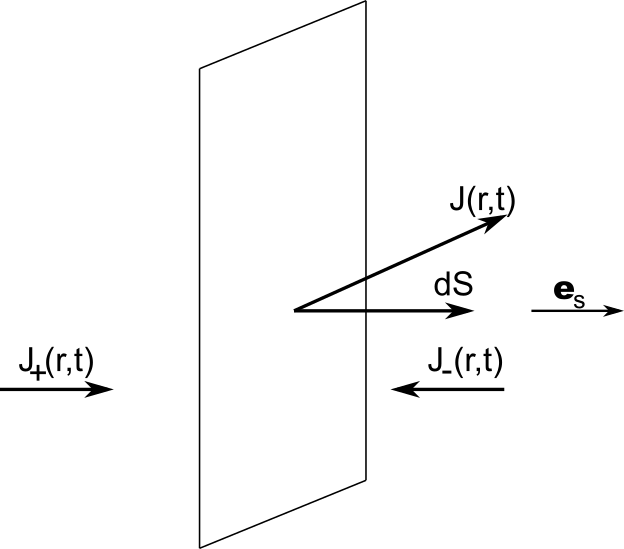
\includegraphics[scale=0.46] {figures/partialcurrent.png}}\protect
\caption{\label{fig:partialcurrent} \footnotesize{Illustration of partial current.}}
\end{figure} 

As a final note we can mention that for isotropy the angular density is independent of $\mathbf{\Omega}$

$$n(\mathbf{r},E,\mathbf{\Omega},t)=\frac{1}{4\pi}N(\mathbf{r},E,t)$$


\subsection{Neutron transport equation}

Let us consider that we selected a beam of neutrons at the location $\mathbf{r}$ in dV, at energy $(E,E+dE)$, and traveling to direction  $\mathbf{d\Omega}$ around $\mathbf{\Omega}$. At time $t$. The number of neutrons in the beam is $n(\mathbf{r},E,\mathbf{\Omega},t)dVdEd\mathbf{\Omega}$.

What happens with this beam after time $dt$? A fraction of the beam will be at $\mathbf{r}+v\mathbf{\Omega}dt$. Another fraction will undergo reactions, and will be lost from the beam. In the meantime other neutrons enter the beam from reactions of other beams. The beam loses neutrons due to scattering out, fission, capture (ie. all the reactions described by the total macroscopic cross section)\footnote{Two other reactions might happen with neutrons, which we can safely neglect: a neutron might beta-decay with a half-life of 12 minutes, which as we will see is much longer than the lifetime of neutrons in a reactor; and in theory neutron-neutron interaction might happen, but these have so long mean free path that we can ignore it, if we couldn't, the developed transport equation would have non linear components, similarly as the equations describing gas transport}. And the beam gains neutrons from fission, in-scattering, or possibly from an external source. Let say the number of such source neutrons is

$$Q(\mathbf{r},E,\mathbf{\Omega},t)dVdEd\mathbf{\Omega}dt$$

\noindent then we can summarize the transport with an equation

\begin{equation}
\Big(n(\mathbf{r}+v\mathbf{\Omega}dt,E,\mathbf{\Omega},t+dt)-n(\mathbf{r},E,\mathbf{\Omega},t)\Big)dVdEd\mathbf{\Omega}=
\end{equation}

\begin{equation*}
=-\Sigma_t(\mathbf{r},E)\phi(\mathbf{r},E,\mathbf{\Omega},t)dVdEd\mathbf{\Omega}dt+Q(\mathbf{r},E,\mathbf{\Omega},t)dVdEd\mathbf{\Omega}dt
\end{equation*}

Let us divide with dt, and assume that $dt\rightarrow 0$, then the left side becomes a total derivative (it is the derivative with respect to time as it would appear to an observer moving with the packet of neutrons). Let's play with that a bit.

\begin{equation}
\frac{dn}{dt}=\frac{n(\mathbf{r}+v\mathbf{\Omega}dt,E,\mathbf{\Omega},t+dt)-n(\mathbf{r},E,\mathbf{\Omega},t)}{dt}
\end{equation}

\begin{equation*}
=\frac{n(\mathbf{r}+v\mathbf{\Omega}dt,E,\mathbf{\Omega},t+dt)-n(\mathbf{r},E,\mathbf{\Omega},t)+n(\mathbf{r},E,\mathbf{\Omega},t+dt)-n(\mathbf{r},E,\mathbf{\Omega},t+dt)}{dt}
\end{equation*}

\begin{equation*}
=\frac{\partial n}{\partial t}+v\mathbf{\Omega}\nabla n
\end{equation*}

\noindent where for simplicity the arguments of the functions were not written, also note that the speed depends on energy $v(E)$. The partial derivative is the change of rate at a fixed position, whereas the total derivative is the change of rate within the packet or beam which is moving. The difference is often called streaming. From the point of view of an observer traveling with the beam, there would be no contribution from streaming. With that the most generic neutron transport equation describing the flux will be.

\begin{equation}
\frac{1}{v}\frac{\partial\phi(\mathbf{r},E,\mathbf{\Omega},t)}{\partial t}=-\mathbf{\Omega}\nabla\phi(\mathbf{r},E,\mathbf{\Omega},t)-\Sigma_t(\mathbf{r},E)\phi(\mathbf{r},E,\mathbf{\Omega},t)+Q(\mathbf{r},E,\mathbf{\Omega},t)
\end{equation}

This equation is called neutron transport equation, or often referred to as Boltzmann-equation\footnote{The reader might notice that Ludwig Boltzmann was not alive when the neutron was discovered, nevertheless he developed similar equations for the kinetic theory of gases, hence the neutron transport equation is also named after him}. In order to expend the source $Q$, we will include the possible sources of neutrons as reaction rates

\begin{equation}
Q(\mathbf{r},E,\mathbf{\Omega},t)=S(\mathbf{r},E,\mathbf{\Omega},t)+
\end{equation}

\begin{equation*}
+\int_{4\pi}\int_{0}^\infty \Sigma_s(\mathbf{r},E')F(E',\Omega' \rightarrow E,\Omega)\phi(\mathbf{r},E',\mathbf{\Omega'},t)d\mathbf{\Omega'}dE'
\end{equation*}

\begin{equation*}
+\frac{\chi(E)}{4\pi}\int_{4\pi}\int_{0}^\infty \nu(E')\Sigma_f(\mathbf{r},E')\phi(\mathbf{r},E',\mathbf{\Omega'},t)d\mathbf{\Omega'}dE'
\end{equation*}

We could include other terms (such as inelastic scattering, or photo-fission), however for LWR applications the role of these reactions is negligible. Of course, there are some initial and boundary conditions. At a free surface (where a neutron return after crossing), characterized by the outward normal $\mathbf{n}$, there is no flux for the incoming direction:

\begin{equation}
\phi(\mathbf{r_b},E,\mathbf{\Omega},t)=0 \: \text{for} \: \mathbf{n\Omega}<0
\end{equation}

Note, there are more heuristic derivations of the transport equation. Those mostly differ by the derivation of this streaming term (the other terms are already heuristic enough). Here we have followed the derivation from the B\&G book. Let us just briefly mention the other type of derivations: in that case there is a gain term due to neutrons streaming into our volume V (bounded by surface S), and a loss term due to neutrons streaming out. We can handle these as a net leakage with the concept of angular current density $\mathbf{j}(\mathbf{r},E',\mathbf{\Omega'},t)$. The rate at which neutrons leak out is:

$$\mathbf{j}(\mathbf{r},E',\mathbf{\Omega'},t)dS=\mathbf{\Omega}\phi(\mathbf{r},E',\mathbf{\Omega'},t)dS$$

\noindent hence the contribution over the whole surface is

$$=\int_S\mathbf{\Omega}\phi(\mathbf{r},E',\mathbf{\Omega'},t)dS=\int_V\mathbf{\Omega}\nabla\phi(\mathbf{r},E',\mathbf{\Omega'},t)dV$$

Notice, that in these derivations one would write up the volume integrals first, and then when all term is a volume integral, drop them. See D\&H p111.

\subsubsection{Possible solutions to the transport equation}

The neutron transport equation is an exact description of the neutron distribution, which yields the angular flux as a solution, which is all the information (or often even more) what we need to study reactors. Let's consider that all the geometry (spatial dependence of the cross sections), and the cross section information is available. Nevertheless, still we find ourselves in some trouble, because

\begin{itemize}
\item we have seven independent variables.
\item the spatial dependence of the cross sections is complicated
\item the energy dependence of cross sections is complicated (resonances, thresholds)
\end{itemize}

In order to solve such an equation, we would need computers, but even so it is too difficult. So, the task is usually, to simplify the transport equation based on reasonable approximations. However this is a topic for more advanced courses. For the moment we would just summarize how the variables could be handled.

Since computers are useful for solving linear algebra, and not calculus, usually the task is to convert this equation into a linear algebra problem. For this we will need to \textit{discretize} the variables and have a discrete representation of derivatives and integrals. For this one can use \textit{discrete ordinates} or \textit{function expansion}.

Let's consider that the general problem is stated as

\begin{equation}
F\Big(f(x),df/dx,d^2f/dx^2,...,\int f(x')dx',...\Big)=0
\end{equation}

\noindent Then tackling this with discrete ordinates would mean:

\begin{itemize}
\item Discretizing the function  $f(x)\rightarrow f(x_i)\equiv f_i, \: i=1,...,N$
\item Replacing the function with a vector $f(x)\rightarrow (f_1,f_2,...,f_N)$
\item Derivatives become finite differences: $df/dx|_{x=x_i}=\Delta f_i/\Delta x_i$
\item Integrals become numerical quadratures: $\int_a^bf(x)dx=\sum_iw_if_i$
\end{itemize} 

\noindent Whereas tackling with function expansion would mean:

\begin{itemize}
\item Expanding the function $f(x)=\sum_lf_lp_l(x)$
\item Replacing the function with a vector $f(x)\rightarrow (f_1,f_2,...,f_N)$
\item Once the expansion coefficients are calculated we can reconstruct the function without interpolation.
\item If we substitute back this form, we can perform the integration, derivation etc. to arrive to an algebraic equation.
\end{itemize}

An example of function expansion is to use Legendre polynomials if the variable ranges between -1 and +1. (eg. for $\mu=cos\vartheta$).

Let's summarize based on these methods how we can handle the variables in the neutron transport equation:

\begin{enumerate}
\item The direction $\mathbf{\Omega}$
\begin{itemize}
\item can be function expanded with Legendre polynomials. This method is often referred to as $P_N$ equations. Usually only low order solutions are used.
\item can be discretized (we select certain rays). This method is often referred to as $S_N$ equations.
\end{itemize}
\item Energy
\begin{itemize}
\item The cross sections and the spectrum has a strong dependence on energy, over a large span (from a fraction of eV to 10 MeV).
\item Thus energy is discretized into energy groups
\item We replace the continuous cross sections with spectrum weighted cross sections: $\Sigma_g=\frac{\int_{E_g}^{E_{g-1}}\Sigma(E)\varphi(E)}{\int_{E_g}^{E_{g-1}}\varphi(E)}$. Note that in order to do so, one needs a knowledge of the neutron spectrum. Therefore calculations are usually split into parts, first solving the slowing down equation on the fuel cell level (pin or assembly), and using the group cross sections in further calculations.
\end{itemize}
\item Space is handled with a spatial mesh.
\item Time is discretized.
\end{enumerate}

Note that it might be a bit counter intuitive that for the weighted cross section the integral bounderies are $E_g - E_{g-1}$. As we saw earlier when neutrons slow down in energy, therefore it is sometimes more convenient to use a reverse labeling as shown in Figure \ref{fig:energygroups}. Since this used in most practical applications and other textbooks, we have also using this.

\begin{figure}[ht!]
\protect \centering{
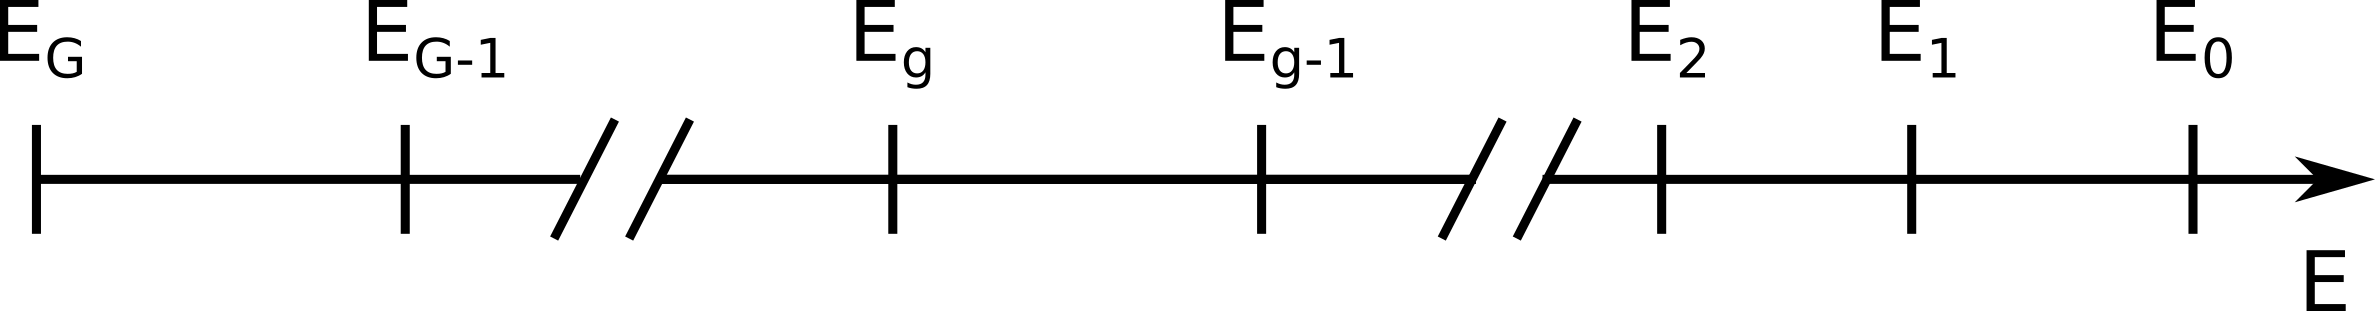
\includegraphics[scale=0.46] {figures/04-energygroups.png}}\protect
\caption{\label{fig:energygroups} \footnotesize{Indexing of energy groups.}}
\end{figure} 


If we were doing a brute force calculation, with 100x100x100 space points, 10 energy groups, 10 directions, we would obtain 10$^8$ equations for each time step, which is difficult to handle even with today's computers. Therefore some physical insight is often needed to eliminate variables. For a example critical system is time independent, thus the time variable can be omitted. The geometry often shows some symmetry, therefore the number of dimensions can be reduced. Or as we will see later, we can apply the diffusion approximation to eliminate angular dependence. Altogether, numerical methods solving the neutron transport are the subject of more advanced computational reactor physics discussions.

\subsection{Neutron diffusion}

We had derived before the exact transport equation:

\begin{equation}
\frac{1}{v(E)}\frac{\partial\phi(\mathbf{r},E,\mathbf{\Omega},t)}{\partial t}=-\mathbf{\Omega}\nabla\phi(\mathbf{r},E,\mathbf{\Omega},t)-\Sigma_t(\mathbf{r},E)\phi(\mathbf{r},E,\mathbf{\Omega},t)+S(\mathbf{r},E,\mathbf{\Omega},t) +
\end{equation}

\begin{equation*}
+\int_{4\pi}\int_{0}^\infty \Sigma_s(\mathbf{r},E')F(E',\Omega' \rightarrow E,\Omega)\phi(\mathbf{r},E',\mathbf{\Omega'},t)d\mathbf{\Omega'}dE'
\end{equation*}

\begin{equation*}
+\frac{\chi(E)}{4\pi}\int_{4\pi}\int_{0}^\infty \nu(E')\Sigma_f(\mathbf{r},E')\phi(\mathbf{r},E',\mathbf{\Omega'},t)d\mathbf{\Omega'}dE'
\end{equation*}

Now we will try to reduce this into something easier to handle. It would be convenient to get rid of $\Omega$ variable, since we usually are less interested in the direction. For example we could integrate around all angles, assume that everything only weakly depends on the angle. We can also assume that the media is isotropic (so $F(E',\Omega' \rightarrow E,\Omega)=F(E'\rightarrow E,\Omega'\Omega)$. We would arrive to%, and we also saw before that for simple elastic, isotropic scattering it doesn't play a role in the scattering kernel (so we assume that scattering is isotropic in LAB, which we know is not true for low $A$). Here I only assume that the media is isotropic (so $F(E',\Omega' \rightarrow E,\Omega)=F(E'\rightarrow E,\Omega'\Omega)$. We would arrive to

\begin{equation}
\frac{1}{v}\frac{\partial\Phi(\mathbf{r},E,t)}{\partial t}=-\nabla \mathbf{J}(\mathbf{r},E,t)-\Sigma_t(\mathbf{r},E)\Phi(\mathbf{r},E,t)+S(\mathbf{r},E,t) +
\end{equation}

\begin{equation*}
+\int_{0}^\infty \Sigma_s(\mathbf{r},E')F(E' \rightarrow E)\Phi(\mathbf{r},E',t)dE'
\end{equation*}

\begin{equation*}
+\chi(E)\int_{0}^\infty \nu(E')\Sigma_f(\mathbf{r},E')\Phi(\mathbf{r},E',t)dE'
\end{equation*}

This is called the neutron continuity equation. However, notice that we have not completely eliminated the direction, since it appears in $\mathbf{J}$. The way eliminating it will in fact be the diffusion approximation, however for the moment we will only try to make this equation a bit more simple. 

Let us handle energy. We can do is to discretize energy and assume that neutrons can travel only with discrete energies. Our options are:

\begin{itemize}
\item forget about energy, and assume that all neutrons travel with the same speed. This is the 1-group approach.
\item Assume that neutrons are either traveling either with thermal or fast energies. This is the 2-group approach
\item Assume that neutrons can have various discrete energies. This is the multi-group approach.
\end{itemize}
    
Again we can mention that the cross sections (and the birth energy spectrum) for the energy groups can be defined as

\begin{equation}
\Sigma_g=\frac{\int_{E_g}^{E_{g-1}}\Sigma(E)\varphi(E)}{\int_{E_g}^{E_{g-1}}\varphi(E)}
\end{equation}
    
Out of these methods the 2-group method is usually used in industrial applications. For the moment we will select the 1-group approach. This rather has an academic relevance: we will be able to solve the diffusion equation analytically, and draw some conclusions on the spatial distribution of neutrons. In case of 1-group, a lot of the quantities and functions will become simpler. Since in case all the neutrons travel with the same speed:

\begin{itemize}
\item then all fission neutrons born in the same energy group: $\chi(E)=1$ 
\item all scattering happens within the same group: $F(E' \rightarrow E)=1$
\item therefore we do not care about the scattering cross section $\Sigma_s$ either. Remember that $\Sigma_t=\Sigma_s+\Sigma_a=\Sigma_s+\Sigma_f+\Sigma_c$, therefore $\Sigma_s-\Sigma_t=-\Sigma_a$
\end{itemize} 

If we take into account all these we reach a more manageable equation (note that now even the speed $v$ is an average value):
    
\begin{equation}
\frac{1}{v}\frac{\partial\Phi(\mathbf{r},t)}{\partial t}=-\nabla \mathbf{J}(\mathbf{r},t)-\Sigma_a(\mathbf{r})\Phi(\mathbf{r},t)+S(\mathbf{r},t) 
+\bar\nu\Sigma_f(\mathbf{r})\Phi(\mathbf{r},t)
\end{equation}


It is time to tackle is the divergence of the current. Here we will assume that neutrons in the system behave like a gas (or like chemicals in solutions), and we apply Fick's law. So the neutrons flow from neutron dense locations to locations with less neutrons (and they follow a random walk, with no directional preference in scattering events).

\begin{equation}
\mathbf{J}=-D\nabla \Phi
\end{equation}

Of course it is fair to ask what is this diffusion coefficient? If we would do a more thorough derivation (see D\&H for example) from the transport equation, we could arrive to

\begin{equation}
D=\frac{1}{3(\Sigma_t+\mu_0\Sigma_s)}=\frac{1}{3\Sigma_{tr}}
\end{equation}

\noindent where we have introduced the transport cross section $\Sigma_{tr}$. Of course we have seen earlier that scattering is anisotropic in the LAB system, especially on light nuclei, therefore the diffusion approximation is not always a terribly good approximation. Nevertheless, it can be patched up with various transport corrections, but this is outside of the scope of this topic. With applying Fick's law we arrive to

\begin{equation}
\frac{1}{v}\frac{\partial\Phi(\mathbf{r},t)}{\partial t}=\nabla D(\mathbf{r})\nabla \Phi(\mathbf{r},t)-\Sigma_a(\mathbf{r})\Phi(\mathbf{r},t)+S(\mathbf{r},t) 
+\bar\nu\Sigma_f(\mathbf{r})\Phi(\mathbf{r},t)
\end{equation}

\noindent where we have considered that the diffusion coefficient $D(\mathbf{r})$ might depend on the location. 

For simplicity, let's assume, that our whole reactor is homogeneous which in practice is not the case - besides for molten salt reactors- because we knew that it is made of heterogeneous structures, such as fuel rods surrounded with coolant. Just think about the fission cross section, which has jumps at the fuel coolant boundaries. But in practical calculations we often spatially homogenize regions. In a homogeneous reactor the cross sections don't depend on the location. 

\begin{equation}
\frac{1}{v}\frac{\partial\Phi(\mathbf{r},t)}{\partial t}=D\nabla^2 \Phi(\mathbf{r},t)-\Sigma_a\Phi(\mathbf{r},t)+S(\mathbf{r},t) 
+\bar\nu\Sigma_f\Phi(\mathbf{r},t)
\end{equation}

And finally let us handle the time dependence. Of course there are several cases of interest: in a non-multiplying system ($\Sigma_f=0$) the last term disappears and in case of a constant source we observe a steady state flux. 

For a multiplying system without a source we can renormalize the fission source term by dividing it with $k$. For a supercritical system $k > 1$, the normalization depresses the fission neutron production rate. For a subcritical system $k < 1$, the normalization increases the fission neutron production rate. Thus after the normalization we would obtain a steady state problem

\begin{equation}
0=D\nabla^2 \Phi(\mathbf{r})-\Sigma_a\Phi(\mathbf{r})+\frac{1}{k}\bar\nu\Sigma_f\Phi(\mathbf{r})
\end{equation}

\noindent as we will see in a moment this steady state, 1-group diffusion equation can be used to investigate the shape of the flux in various geometries, and to find conditions for criticality.

\subsubsection{Limitations of diffusion theory and other comments}

We have pointed out that the diffusion theory has certain limitations, let us summarize these:

\begin{itemize}
\item The anisotropy of flux will depend on location. If we are far from absorbers (control rods) and from locations where the spatial dependence of the flux is strong, then we can assume that the flux just weakly depends on the direction.

\item Time dependence: we neglected the time derivative. If we wouldn't have done it, then the diffusion coefficient would have an $\omega/v$ "time absorption cross section". But for most processes in a reactor we can neglect this.

\item The anisotropy of the scattering kernel: we have seen that for light nuclei the LAB scattering is anisotropic even for isotropic CM scattering. 
\end{itemize}

Note that the diffusion theory and the diffusion coefficient can be derived directly from transport theory by the expansion of the scattering kernel and the flux with spherical harmonics (the derivation is outside of the lecture, but you can find it in D\&H):

$$\phi(\mathbf{r},E,\mathbf{\Omega},t)=\frac{1}{4\pi}\phi(\mathbf{r},E,t)+\frac{3}{4\pi}\mathbf{\Omega}\mathbf{J}(\mathbf{r},E,t)+...$$

and

$$\Sigma_s(\mathbf{r},E'\rightarrow E,\mathbf{\Omega\Omega}')=\frac{1}{4\pi}\Sigma_{s0}(\mathbf{r},E'\rightarrow,E)+\frac{3}{4\pi}\Sigma_{s1}(\mathbf{r},E'\rightarrow,E)\mathbf{\Omega\Omega}'$$

\subsubsection{Diffusion length}

We can rearrange the diffusion equation by introducing various constants (see the Lewis book), for example by introducing

$$\bar\nu\Sigma_f=\Sigma_a\frac{\bar\nu\Sigma_f}{\Sigma_a}=k_\infty\Sigma_a$$

\noindent and the diffusion length

$$L=\sqrt{\frac{D}{\Sigma_a}}$$

\noindent one arrives to

\begin{equation}
0= \nabla^2 \Phi(\mathbf{r})-\frac{k_\infty-1}{L^2}\Phi(\mathbf{r})+\frac{S(\mathbf{r})}{D}
\end{equation}

The diffusion length $L$ (and the diffusion area $L^2$) have physical interpretations. (See Lewis p154). The average length of one single section in the zigzag would be $\Sigma_t$. But the diffusion length is proportional to the root mean square distance diffused by a neutron between birth and absorption as illustrated in Figure \ref{fig:diffusionlength}.

\begin{figure}[ht!]
\protect \centering{
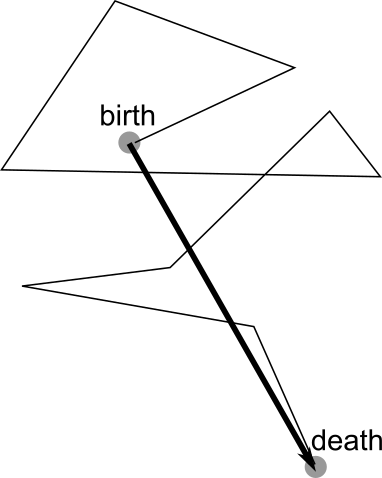
\includegraphics[scale=0.46] {figures/diffusion_length.png}}\protect
\caption{\label{fig:diffusionlength} \footnotesize{Illustration of the diffusion length.}}
\end{figure} 

\subsubsection{Solution to the diffusion equation in simple geometries}

Let us briefly solve the diffusion equation for three simple, homogeneous geometries. In D\&H you can find the derivation for other geometries as well.

\subsubsection*{1D multiplying slab}

If we rearrange the equation we arrive to the Helmholtz-equation

\begin{equation}
-\frac{\nabla^2 \Phi}{\Phi}=\frac{\frac{1}{k}\bar\nu\Sigma_f-\Sigma_a}{D}
\end{equation}

Or by introducing a new constant which depends on the materials of the reactor.

\begin{equation}
\nabla^2 \Phi+B_m^2\Phi=0
\end{equation}

Our trial solution is $\Phi(x)=A\cos Bx+C\sin Ex$. We know that the flux is symmetric, so  $d\Phi/dx|_{x=0}=0$, which leaves the cosine term. Let's substitute that to the original equation

\begin{equation}
-\frac{-AB^2cosBx}{AcosBx}=B^2=\frac{\frac{1}{k}\bar\nu\Sigma_f-\Sigma_a}{D}
\end{equation}

Clearly now we have used a $B^2$ which only depends on the geometry. Let's call it $B_g^2$, the geometry buckling factor. We can determine it from the boundary condition. Let's consider that the flux disappears at edges of the slab at $x=a$ and $x=-a$ (so the size of the reactor is $2a$)

\[
B_ga=\frac{\pi}{2} \rightarrow B_g=\frac{\pi}{2a}
\]

Of course, at the edge of the reactor the flux should not become zero if the slab is surrounded with vacuum as this is highlighted in Figure \ref{fig:boundary} A more meaningful boundary condition could be introduced through the partial currents. From Fick's law we could derive (see D\&H)

\begin{figure}[ht!]
\protect \centering{
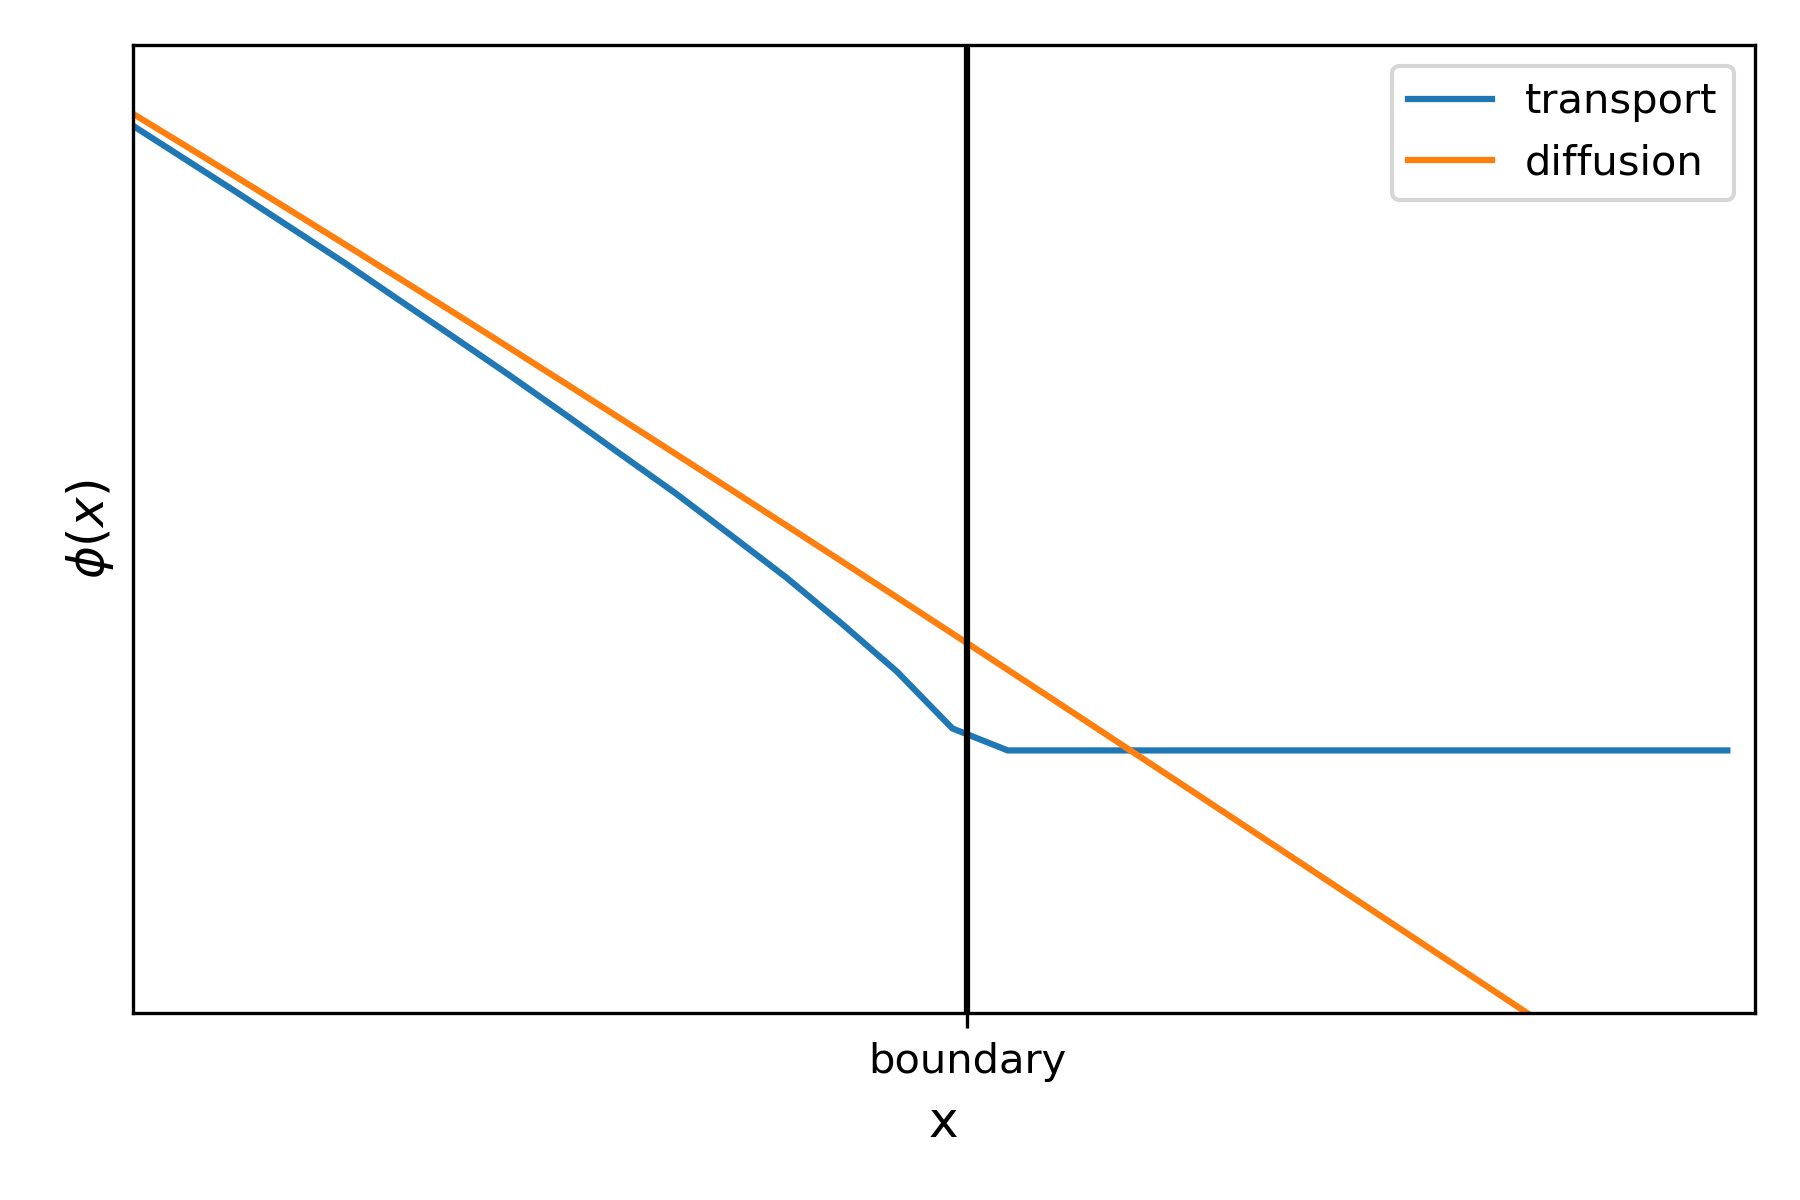
\includegraphics[scale=0.46] {figures/04-vacuumboundaries.png}}\protect
\caption{\label{fig:boundary} \footnotesize{Vacuum boundaries in transport and diffusion theory. One can observe that we need to "extrapolate" the boundary for diffusion.}}
\end{figure} 


\[
J_x^\pm=\frac{1}{4}\Phi\mp\frac{1}{2}D\frac{d}{dx}\Phi
\]

And we know that for a vacuum boundary $J_x^-(a)=0$, from which we find that the flux should become zero at $a+2D$ (and based on transport equation even more accurate results could be obtained). This doesn't mean that the flux is physically zero at this location, since if the slab is surrounded by vacuum, the flux after the edge is going to be constant. It means that mathematically speaking if the flux would be extrapolated it should disappear at $a+2D$. In the following we will always assume "extrapolated boundaries", so we don't need to worry about this.

\begin{figure}[ht!]
\protect \centering{
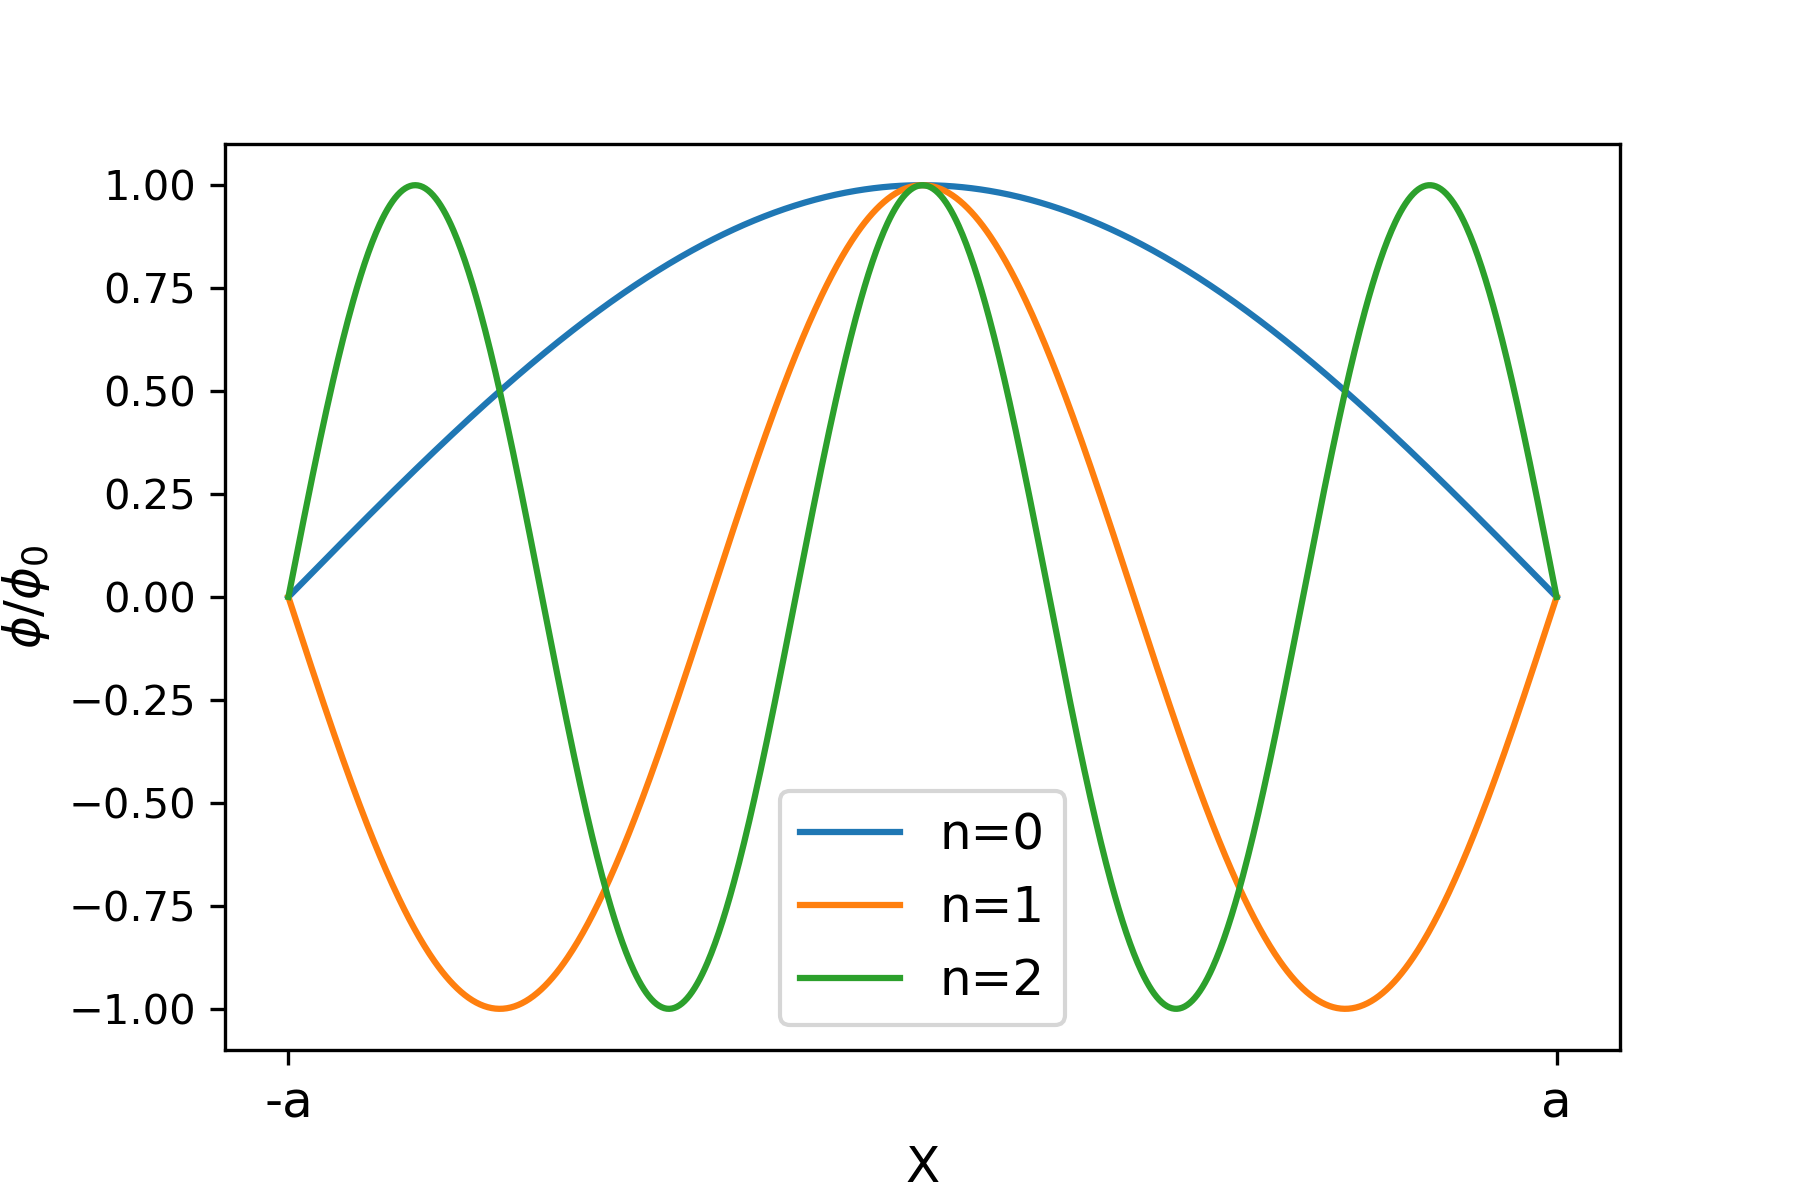
\includegraphics[scale=0.46] {figures/04-slabflux.png}}\protect
\caption{\label{fig:multislab} \footnotesize{Mathematically correct solutions to the diffusion equation in a slab. $n=0$ is the fundamental mode.}}
\end{figure} 

Note that the Helmoltz equation produces valid solutions at $B_{g,n}a=\frac{\pi}{2}+n\pi$, so $B_{g,n}=\frac{(2n+1)\pi}{2a}$. However those will not be physical, so we keep the $n=0$ fundamental mode, as shown in Figure \ref{fig:multislab}, and for this course we don't care about the other modes.

For a critical reactor $k=1$, the constant $B_m^2$ becomes

$$B_m^2=\frac{\bar\nu\Sigma_f-\Sigma_a}{D}$$

\noindent and as mentioned earlier it only depends on the materials of the reactor. Therefore, we will call it the material buckling factor. It is clear that the condition of criticality is

\begin{equation}
B_g^2=B_m^2
\end{equation}

But it is also apparent, that in case we know the the material and the geometry buckling, we can figure out the $k$:

\begin{equation}
k=\frac{\bar\nu\Sigma_f}{DB_g^2+\Sigma_a}=\frac{\text{gains}}{\text{losses}}
\end{equation}

\noindent and this results is aligned with our previous, intuitive definition of the multiplication factor, since it is a ratio of the gains and losses of neutrons.

We can use this result to perform some basic investigations. What happens if

\begin{itemize}
\item we introduce more absorber and increase $\Sigma_a$? Then $k$ goes down.
\item we increase the size of the reactor? Then $B_g$ decreases, thus $k$ increases. 
\item we increase the temperature $T$? This is a bit more complicated question, in general we can say that the density goes down, so the number density goes down, so the macroscopic cross sections decrease. Reactor might expand, although usually, this will play only a small role. The diffusion coefficient $D$ increases (since in the denominator, the macroscopic cross sections go down): the atoms are more spread out, so neutrons can move around more easily. But as a summary, we cannot answer the question, since it depends on the exact composition of materials. 
\end{itemize}

One might ask also, where is the power in these solutions? We see that the constant describing the magnitude of the flux $A$ disappeared. Indeed, criticality doesn't depend on the power. That is just a normalization factor. We can have even (almost) zero power reactors (few watts). We can obtain the normalization factor $A$ from the power:

\begin{equation}
P=\int_V dr^3 w_f\Sigma_f\phi(r)
\end{equation}

\noindent where $w_f$ is the useful energy released in fission.

\subsubsection*{2D Cylindric reactor}

Let's assume that the flux is symmetric in $\varphi$, then the Laplace operator becomes


\[
\frac{1}{r}\frac{\partial}{\partial r}(r\frac{\partial}{\partial r})+\frac{\partial^2}{\partial z^2}
\]

Then, we will separate the variables:

\[
\Phi(r,z)=R(r)Z(z)
\]

\noindent after substituting these in the diffusion equation we arrive to

\[
Z(z)\frac{1}{r}\frac{\partial}{\partial r}(r\frac{\partial}{\partial r}R(r))+R(r)\frac{\partial^2}{\partial z^2}Z(z)=-B^2\Phi(r,z)
\]

\noindent where we can divide by $\Phi(r,z)$:

\[
\frac{1}{R(r)}\frac{1}{r}\frac{\partial}{\partial r}(r\frac{\partial}{\partial r}R(r))+\frac{1}{Z(z)}\frac{\partial^2}{\partial z^2}Z(z)=-B^2
\]

\noindent where we obtain the sum of some function $f(r)$ and $g(z)$, which is constant for all r and z. This is only possible if the two terms are also constant:


\[
\frac{1}{R(r)}\frac{1}{r}\frac{\partial}{\partial r}(r\frac{\partial}{\partial r}R(r))=-B_r^2
\]

\noindent and

\[
\frac{1}{Z(z)}\frac{\partial^2}{\partial z^2}Z(z)=-B_z^2
\]

\noindent and with that

\[
B_r^2+B_z^2=B^2
\]

The equation for the the axial dimension is exactly what we just had for the 1D slab, and in the general solution with the same thinking we can keep only the cosine 

\[
Z(z)=c_1\cos B_zz
\].  

\noindent and by considering that the height of the reactor is $H$ (extrapolated), we arrive to

\[
Z(z)=c_1cos(\frac{\pi}{H}z)
\]

For the radial dimension we need to consult our math books, and find that the function which could fulfill this equation is the Bessel function $J_0(B_rr)$. In fact, similarly as before here also the first and second kind Bessel functions would be solutions, but we drop the second kind to get positive values at $r=0$ as it is shown in Figure \ref{fig:cylinder}.

\[
R(r)=c_2J_0(\frac{2.405}{R}r)
\]

\noindent and with that the final solution is

\[
\Phi(r,z)=c\cos(\frac{\pi}{H}z)J_0(\frac{2.405}{R}r)
\]

\begin{figure}[ht!]
\protect \centering{
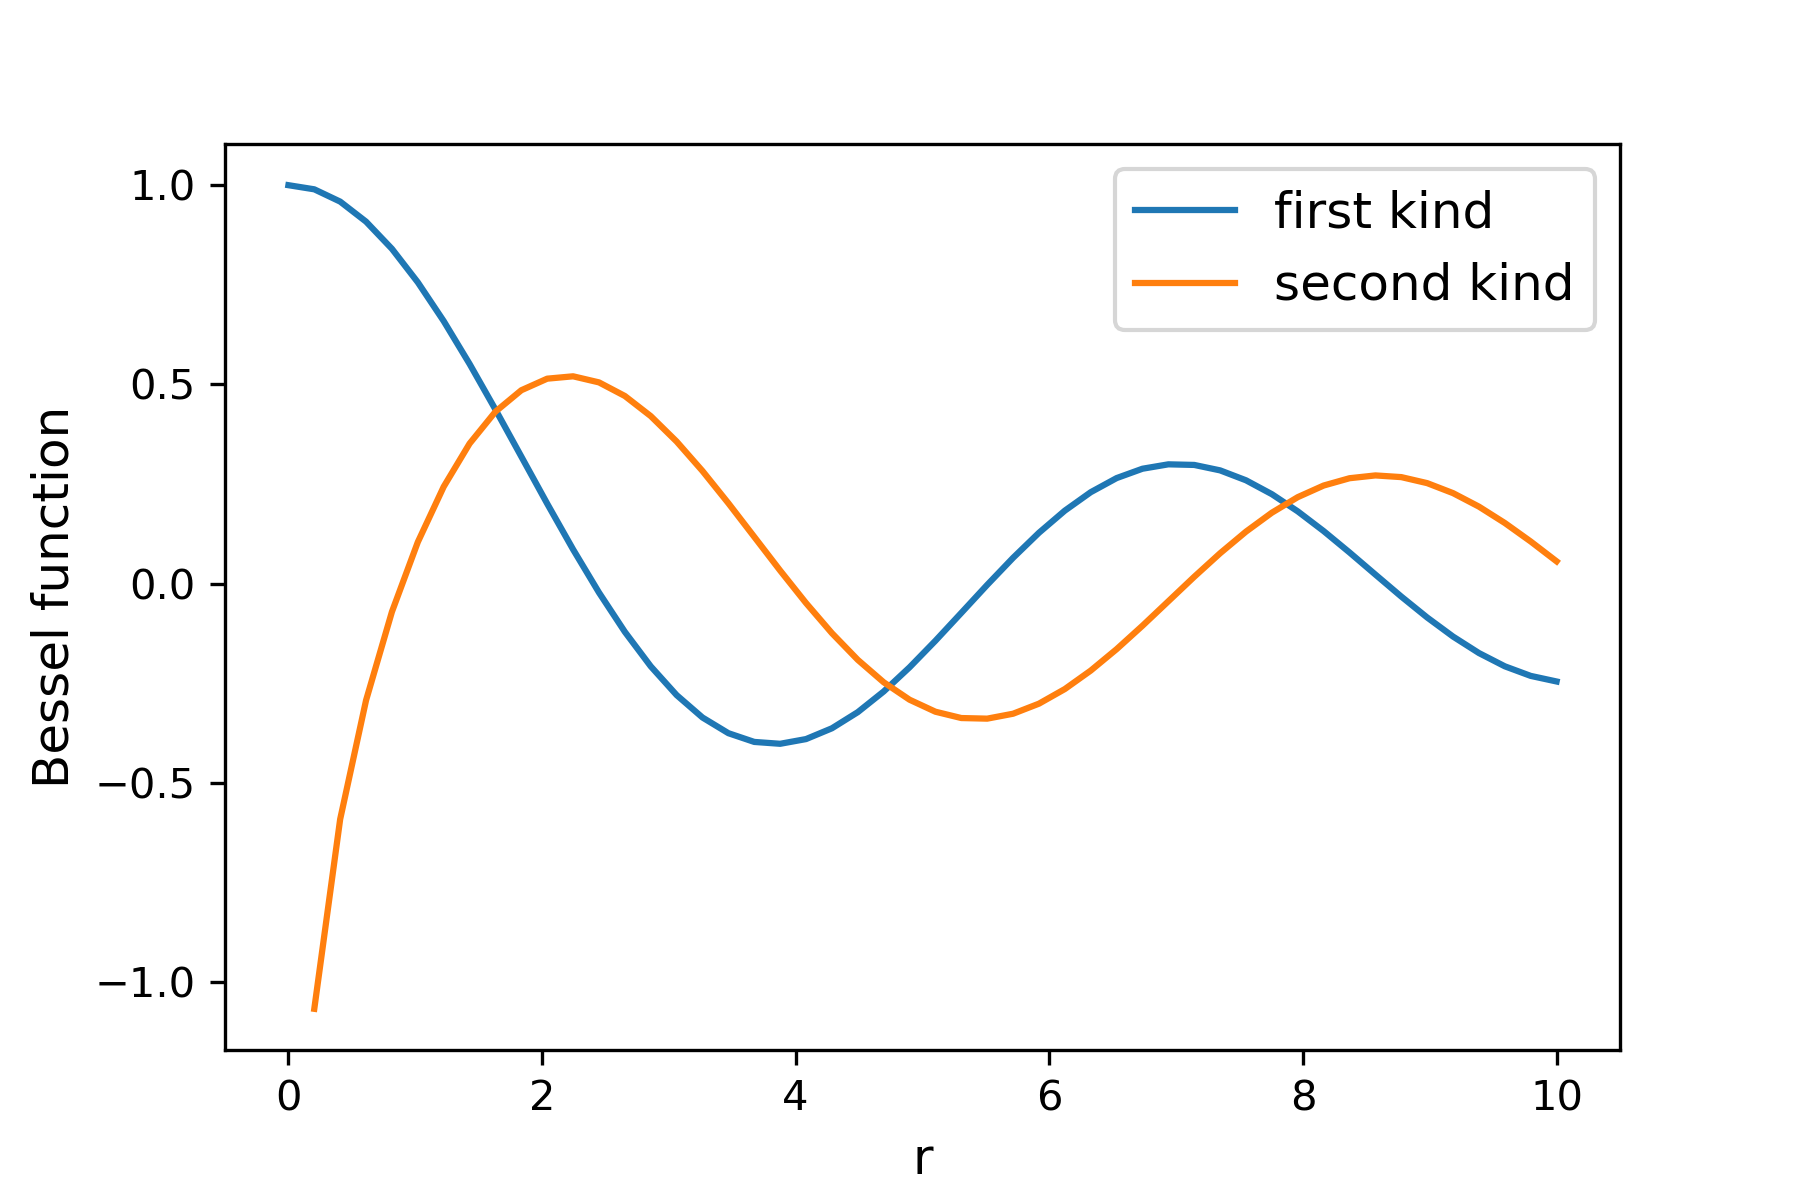
\includegraphics[scale=0.42] {figures/04-besselfunction.png} 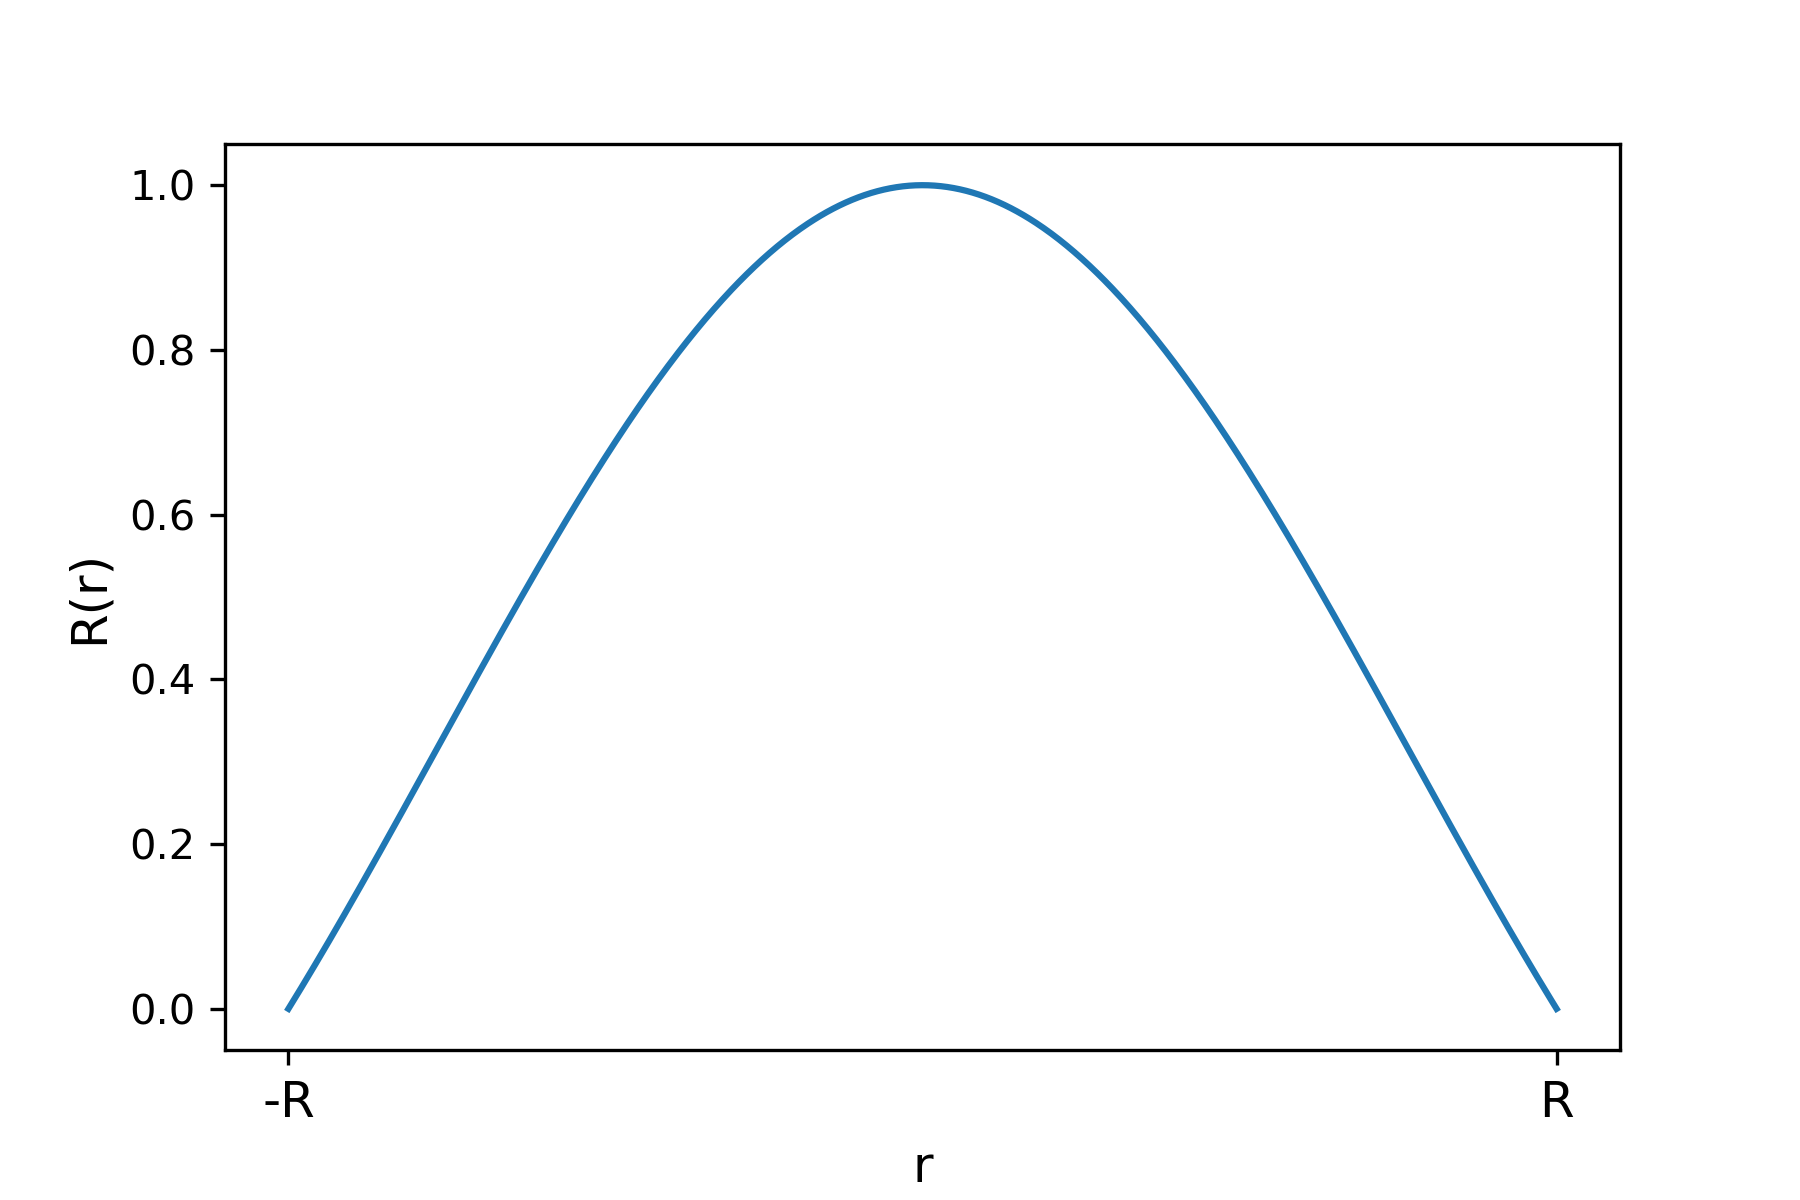
\includegraphics[scale=0.42] {figures/04-cylinderradialflux.png}}\protect
\caption{\label{fig:cylinder} \footnotesize{Illustration of the Bessel-functions and the radial flux profile of a cylinder.}}
\end{figure} 

\subsubsection*{1D non-multiplying slab}

Let us review a case when the material is not multiplying. Then we can obtain a steady case only if there is a source placed in the geometry. Consider a slab, with a planar source placed at the center. The diffusion equation reduces to the one-dimensional form

$$\frac{d^2\phi}{dx^2}-\frac{1}{L^2}\phi=-\frac{S(x)}{D}=-\frac{S_0}{D}\delta(x)$$

where the diffusion length $L=\sqrt{D/\Sigma_a}$ is introduced. Note that in case $x\neq 0$, the equation is even simpler:

$$\frac{d^2\phi}{dx^2}-\frac{1}{L^2}\phi=0$$

We will try to solve this homogeneous equation first, and then use some boundary conditions to get the generic solution.

One boundary condition will be

$$-D\frac{d\phi}{dx}\rvert_{+\epsilon}+D\frac{d\phi}{dx}\rvert_{-\epsilon}=J_x(0^+)-J_x(0^-)=S_0$$

and due to the symmetry of the geometry

$$J_x(0^+)=-J_x(0^-)=J(0)$$

thus the first boundary condition is

$$\mathrm{lim}_{x\rightarrow 0^+} -D\frac{d\phi}{dx}=\frac{S_0}{2}$$

\noindent thus the net current at the origin at either side must be half of the source strength.

Since we have a second order derivative we need and other boundary condition as well: we will use the condition of finite flux as $x\rightarrow \infty$:

$$\mathrm{lim}_{x\rightarrow \infty} \phi(x) < \infty$$

We solve for the positive side, and then infer symmetry for the negative side. The general solution is

$$\phi(x)=A\cdot\exp\Big(-\frac{x}{L}\Big)+B\cdot\exp\Big(\frac{x}{L}\Big)$$

\noindent where due to the second BC $B=0$. And due to the first BC

$$\mathrm{lim}_{x\rightarrow 0^+} -D\Bigg(-\frac{A}{L}\cdot\exp\Big(-\frac{x}{L}\Big)\Bigg)=\frac{AD}{L}=\frac{S_0}{2} \rightarrow A=\frac{S_0L}{2D}$$

\noindent thus the solution is (illustrated in Fig. \ref{fig:nonmultislab}).

$$\phi(x)=\frac{S_0L}{2D}\cdot\exp\Big(-\frac{|x|}{L}\Big)$$


\begin{figure}[ht!]
\protect \centering{
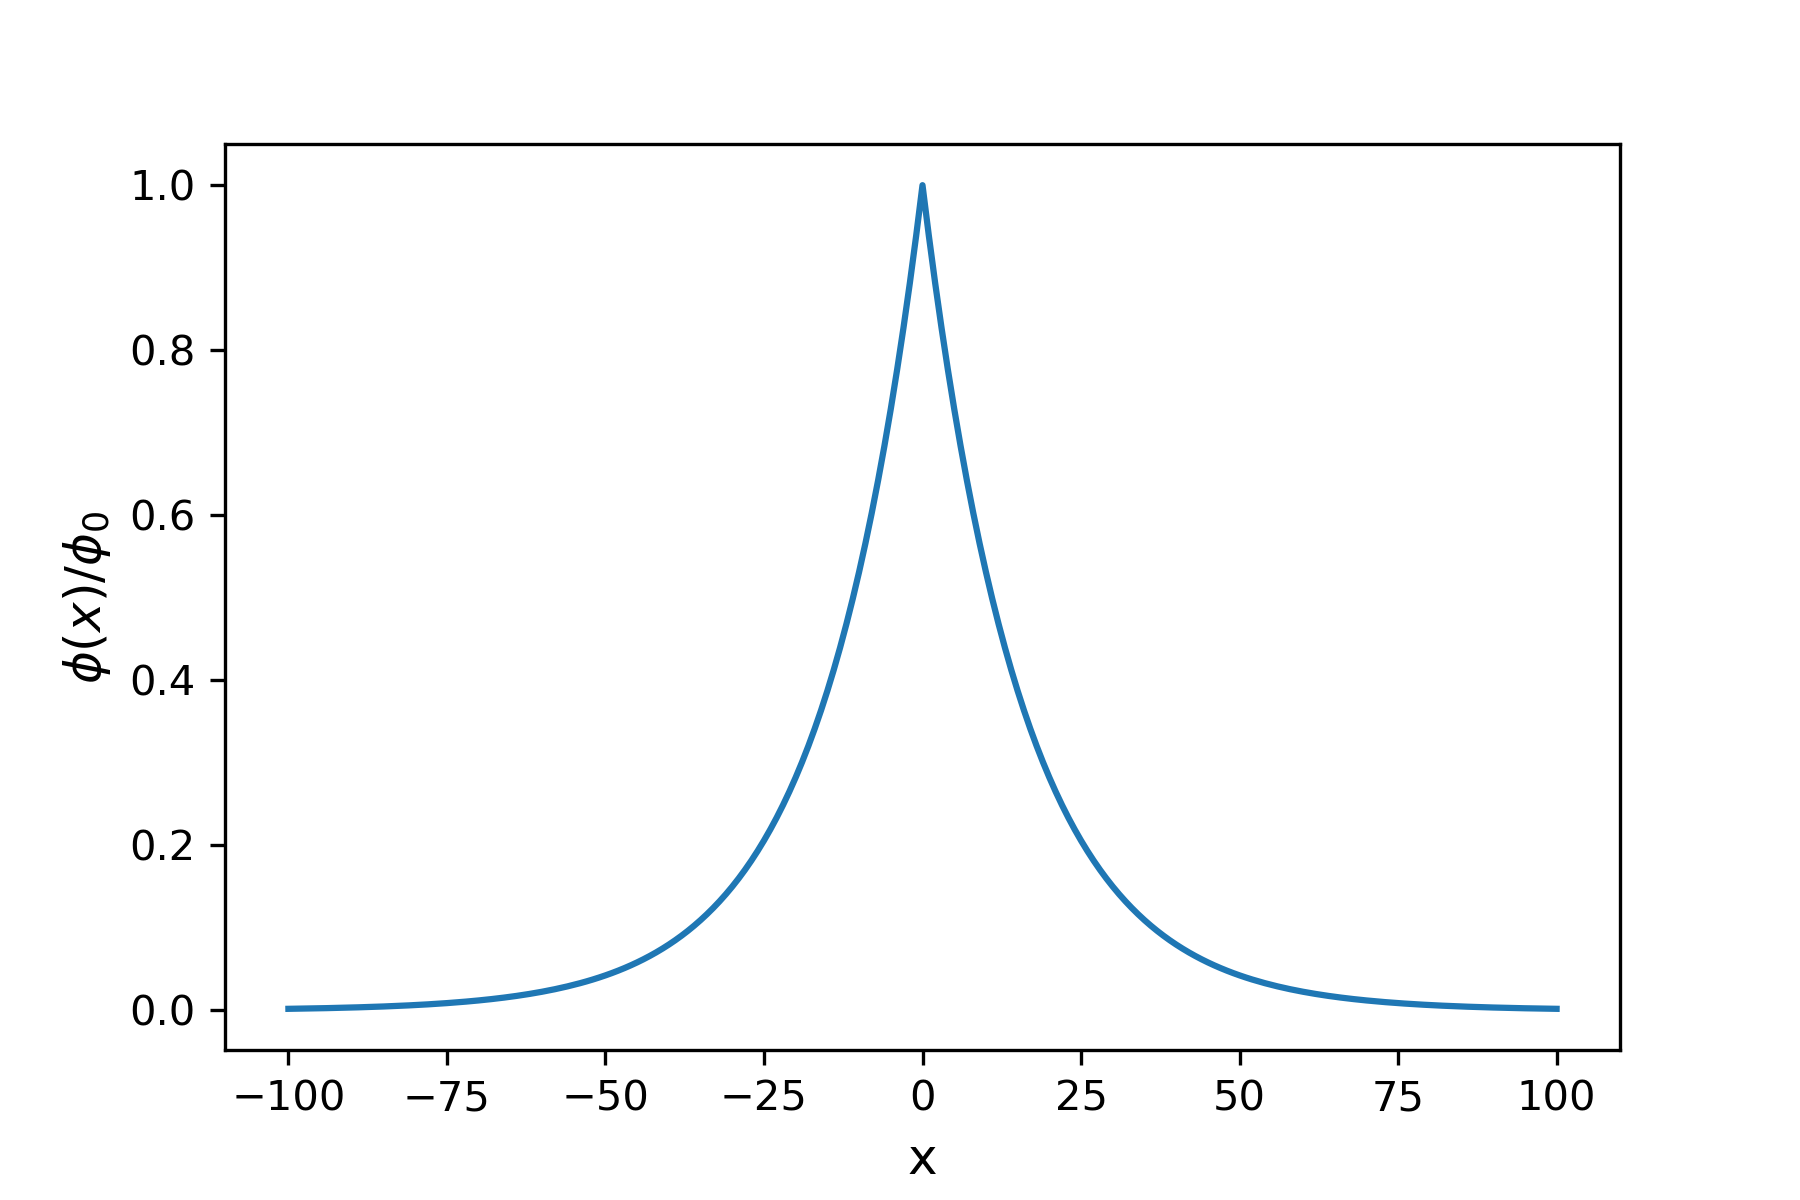
\includegraphics[scale=0.46] {figures/04-nonmultislab.png}}\protect
\caption{\label{fig:nonmultislab} \footnotesize{Solution to the flux in a nonmultiplying slab.}}
\end{figure} 

\subsection{Reflected geometries}

In practice the reactor is of course not surrounded with vacuum, but typically with some material which can scatter neutrons. This can mean, that the reactor core is surrounded with water, but in fast reactors often the core is surrounded with so called reflector assemblies (since the coolant would not reflect neutrons). The main reason of doing so is to reduce the leakage of neutrons.

One could derive the flux shape for a reflected geometry. We will omit the derivation in the notes (see D\&H p211), just highlight that the criticality condition $B_g^2=B_m^2$ does not hold anymore. The flux shape is shown in Fig. \ref{fig:reflected} (top), the drop of the flux inside the reflector region will depend on the properties of the material. In case the absorption cross section of the material is high the flux quickly goes to zero (of course in that case we do not talk about a reflector anymore, rather an absorber or shield. 

\begin{figure}[ht!]
\protect \centering{
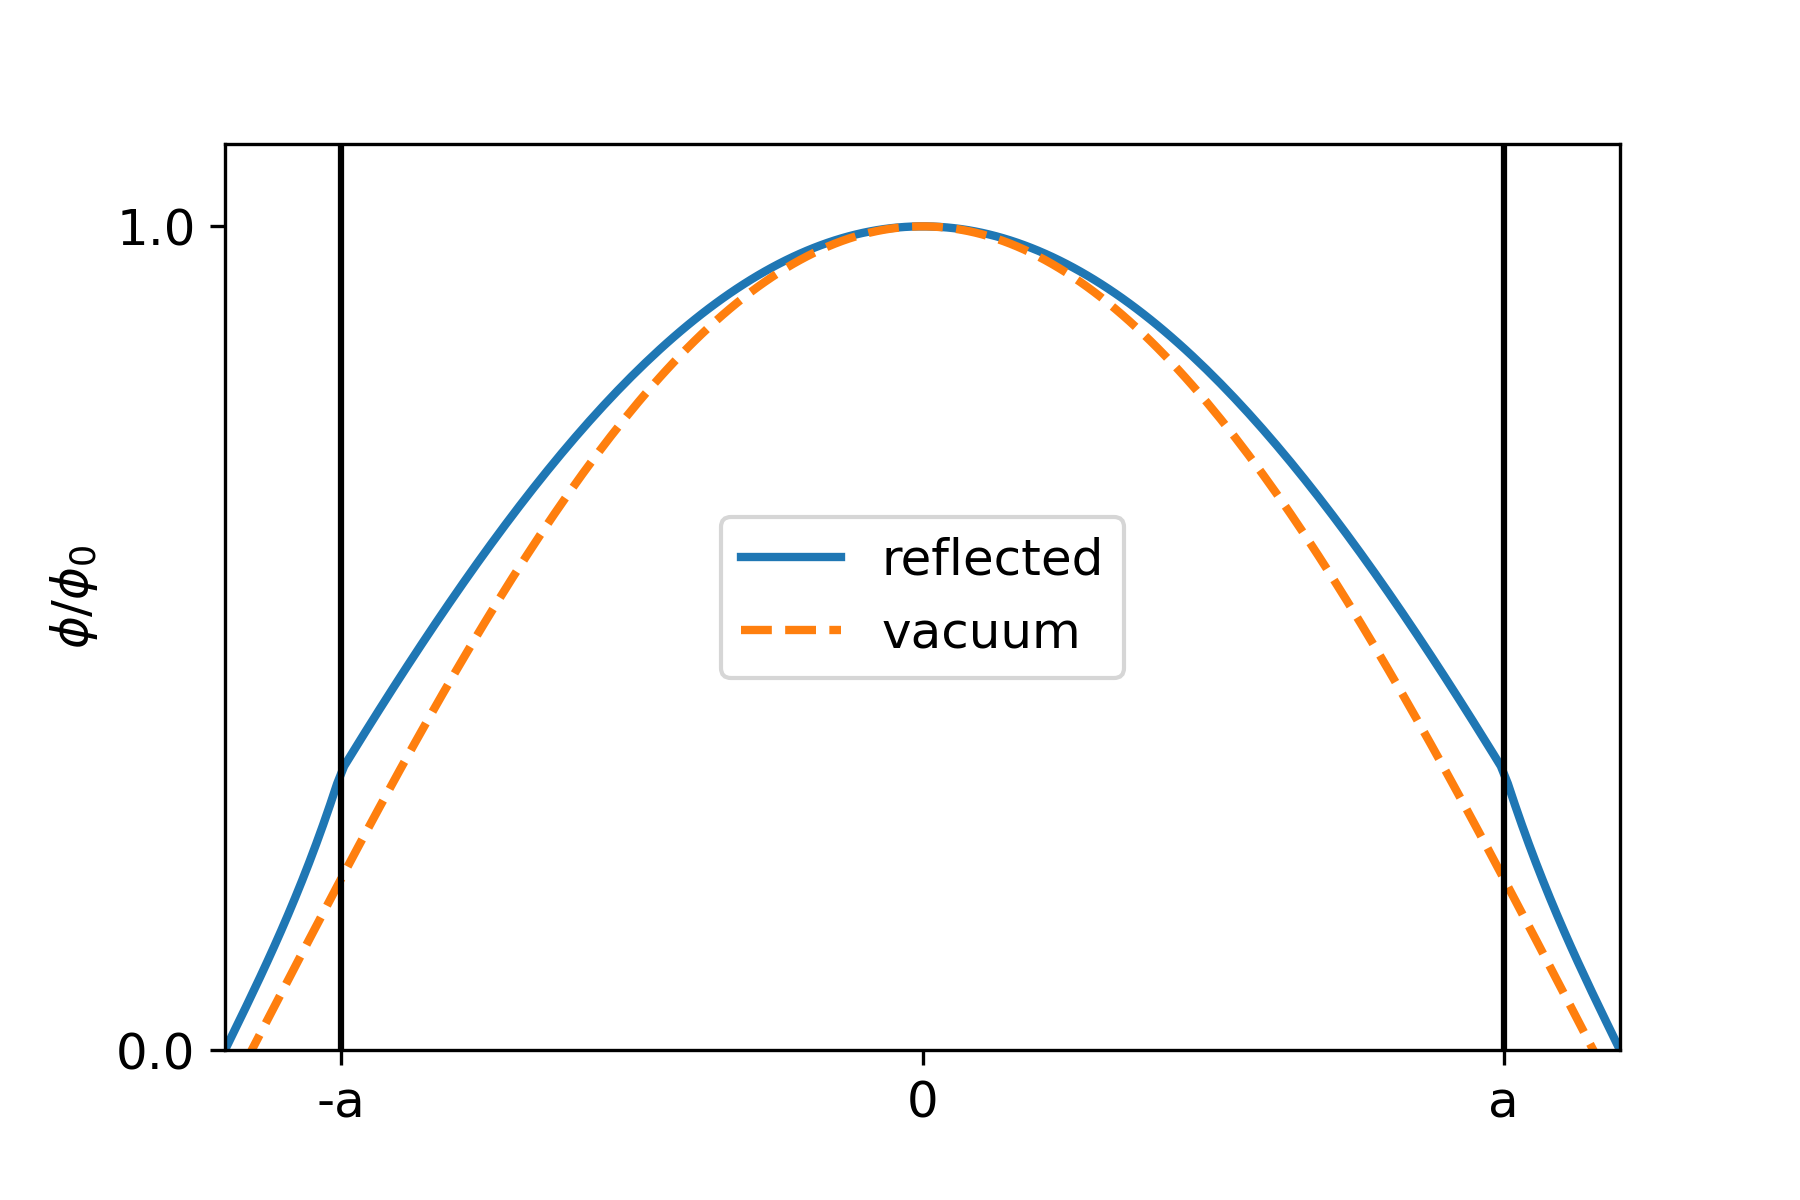
\includegraphics[scale=0.46] {figures/04-reflectedslab_Diffusion.png} 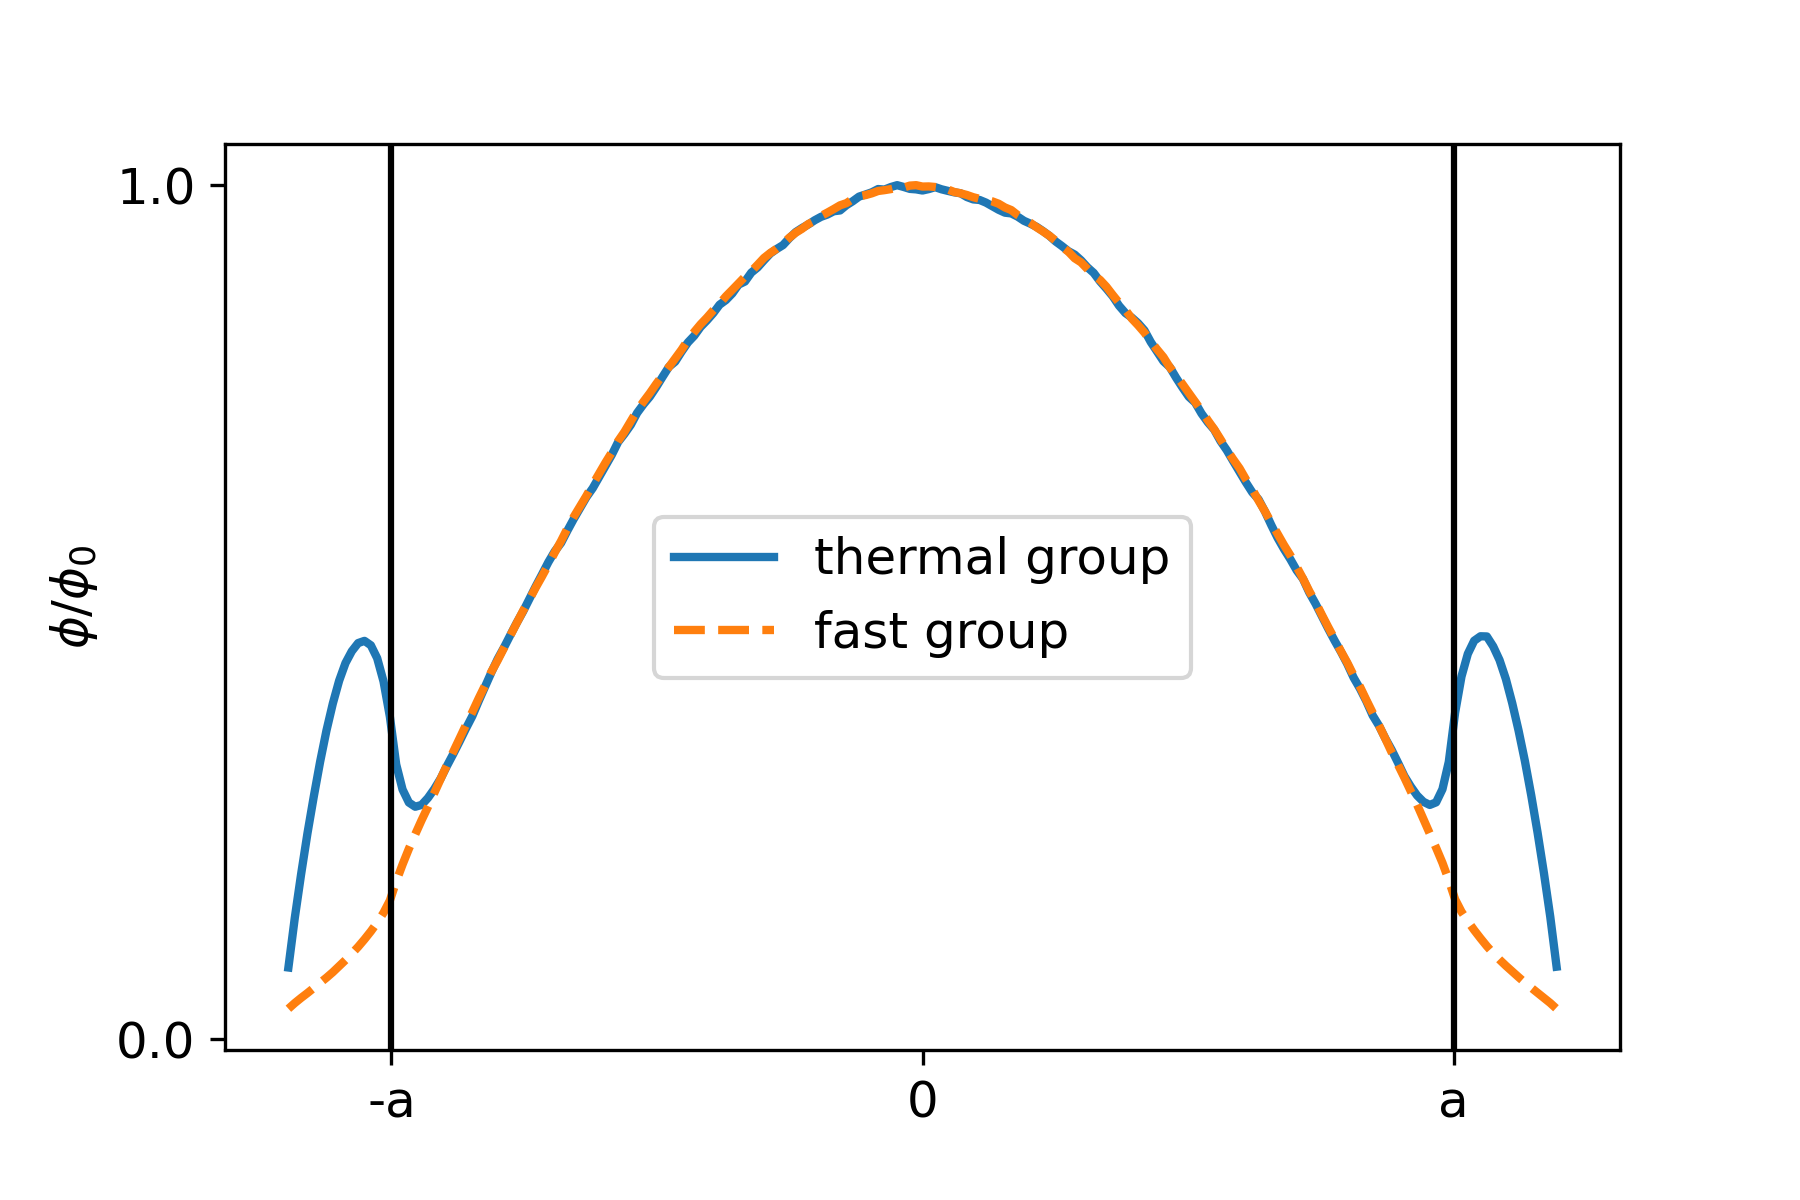
\includegraphics[scale=0.46] {figures/04-reflectedslab_MC.png}}\protect
\caption{\label{fig:reflected} \footnotesize{Spatial distribution of the neutron flux in a reflected slab. Top 1-group diffusion theory. Bottom Monte Carlo particle transport results.}}
\end{figure} 

However, this is a geometry for which our academic tool, the 1-group method gives a rather bad approximation. Namely, that reflected geometries besides reducing leakage also serve to flatten the flux and the power distribution. As a result of this one could observe a peaking of the thermal flux close to the boundary between the core and the reflector as shown in the bottom of Figure \ref{fig:reflected}. However, one needs to apply at least 2-group theory to analyze this effect.

Since reflectors reduce leakage, the fissile core can have a smaller size to achieve criticality. This is called the reflector savings

\begin{equation}
\delta = a_{bare}-a_{reflector}
\end{equation}

\noindent which can be derived as a function of the reflector savings (D\&H p214). Figure \ref{fig:reflectorsavings} illustrates this. The figure indicates how much the critical size can be decreased when the reflector is added. As one would expect intuitively, the function saturates (at around $b=3L_r$), which means that after a certain reflector thickness the critical size of the core cannot be reduced, since neutrons will not reach to and scattered back from such a far distance.

\begin{figure}[ht!]
\protect \centering{
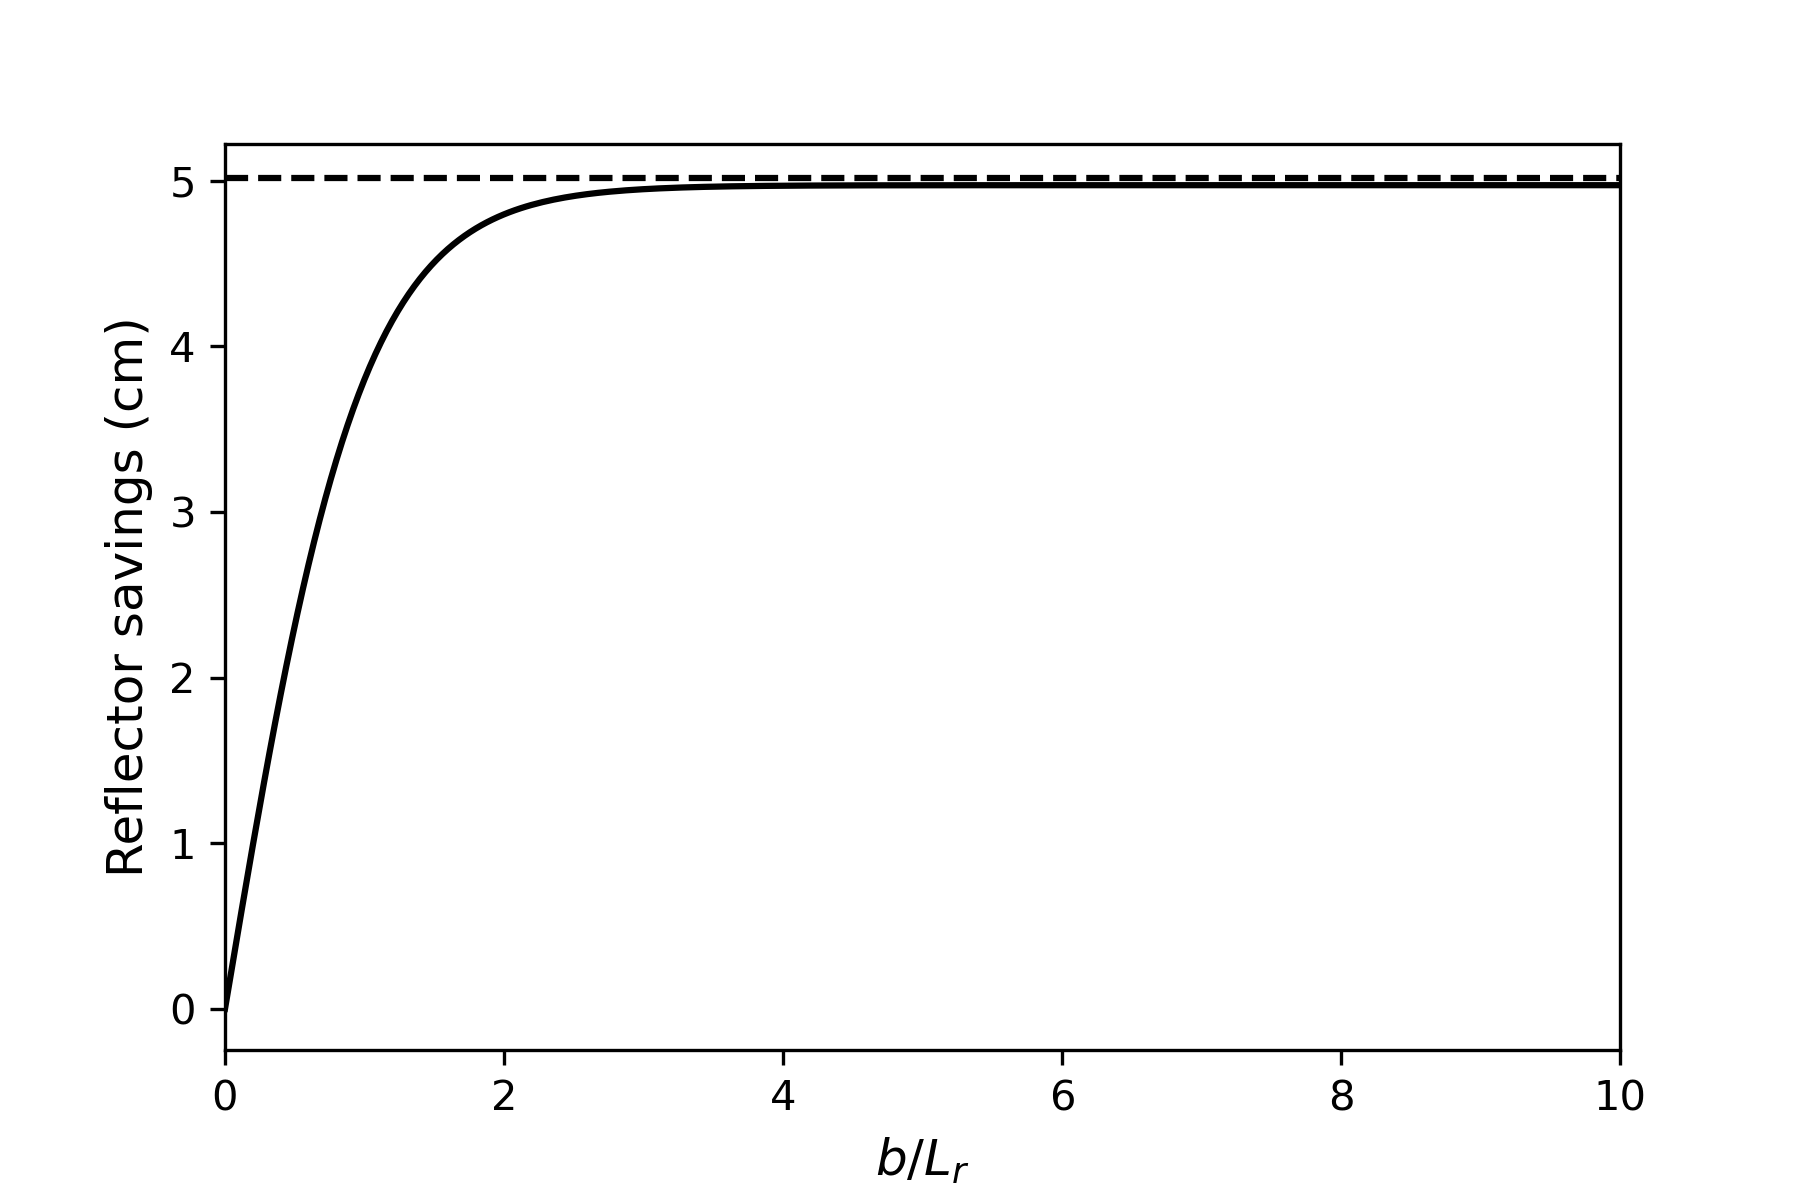
\includegraphics[scale=0.46] {figures/04-reflectorsavings.png}}\protect
\caption{\label{fig:reflectorsavings} \footnotesize{Reflector savings.}}
\end{figure} 

\subsection{2 and Multi group diffusion}

As we saw from the reflected geometry, the 1-group diffusion theory cannot adequately capture all physical phenomena, thus in practice at least 2, but often more groups are used. Within this course we do not intend to solve the 2-group problem analytically, or to implement multi-group numerical solvers, we will only draft the idea behind multigroup methods by developing a 2-group equation.

In 2-group theory the energy boundaries are selected so that there is no upscattering from the thermal to the fast group. The typical boundaries are $E_2=0$, $E_1=1 eV$, $E_0=10 MeV$. In such group structure, we can assume that all the fission event contribute as a source only to the fast group, therefore $\chi_t=0$ and $\chi_f=1$.

Let us summarize the gain and loss term in each of the groups (index $f$ refers to the fast group, and $t$ refers to the thermal group; when double indexes are encountered such as in $\Sigma_{f,t}$, the first term refers to the physical process, such as fission in this example, and the second to the energy group, such as thermal in this example).


\begin{tabular}{c | c | c}
group & Gains & Losses \\
\hline
fast & $\frac{1}{k}\nu_t\Sigma_{f,t}\Phi_t+\frac{1}{k}\nu_f\Sigma_{f,f}\Phi_f$ & $\Sigma_{a,f}\Phi_f + \Sigma_{s,f\rightarrow t}\Phi_f + D_fB_g^2\Phi_f$  \\
\hline
thermal & $\Sigma_{s,f\rightarrow t}\Phi_f$ & $\Sigma_{a,t}\Phi_t  + D_tB_g^2\Phi_t$ 
\end{tabular}

The sources of neutrons in the fast group are both from thermal and fast fission. The sources is of neutrons in the thermal group are only from downscattering from the fast group. Both energy groups lose neutrons due to absorption and leakage, however the downscattering appears as a loss in the fast group.

With these source and loss terms it is possible to develop a coupled set of balance equation for each groups.

\begin{equation}
\frac{1}{k}\nu_t\Sigma_{f,t}\Phi_t+\frac{1}{k}\nu_f\Sigma_{f,f}\Phi_f=\Sigma_{a,f}\Phi_f + \Sigma_{s,f\rightarrow t}\Phi_f + D_fB_g^2\Phi_f 
\end{equation}

\begin{equation*}
\Sigma_{s,f\rightarrow t}\Phi_f = \Sigma_{a,t}\Phi_t  + D_tB_g^2\Phi_t
\end{equation*}


By rearranging the second, we get an expression for the thermal flux

\begin{equation}
\Phi_t=\frac{\Sigma_{s,f\rightarrow t}\Phi_f}{\Sigma_{a,t}  + D_tB_g^2}
\end{equation}

\noindent which can be substituted into the first one

\begin{equation}
\frac{1}{k}\nu_t\Sigma_{f,t}\frac{\Sigma_{s,f\rightarrow t}\Phi_f}{\Sigma_{a,t}  + D_tB_g^2}+\frac{1}{k}\nu_f\Sigma_{f,f}\Phi_f=\Sigma_{a,f}\Phi_f + \Sigma_{s,f\rightarrow t}\Phi_f + D_fB_g^2\Phi_f
\end{equation}

\noindent Then after dividing by $\Phi_f$, one can rearrange for $k$.

\begin{equation}
k=\frac{\nu_t\Sigma_{f,t}\frac{\Sigma_{s,f\rightarrow t}}{\Sigma_{a,t}  + D_tB_g^2}+\nu_f\Sigma_{f,f}}{\Sigma_{a,f} + \Sigma_{s,f\rightarrow t} + D_fB_g^2}=\frac{\text{gains}}{\text{losses}}
\end{equation}

And notice that similarly as before, we could identify the terms as gains and losses.


\begin{figure}[ht!]
\protect \centering{
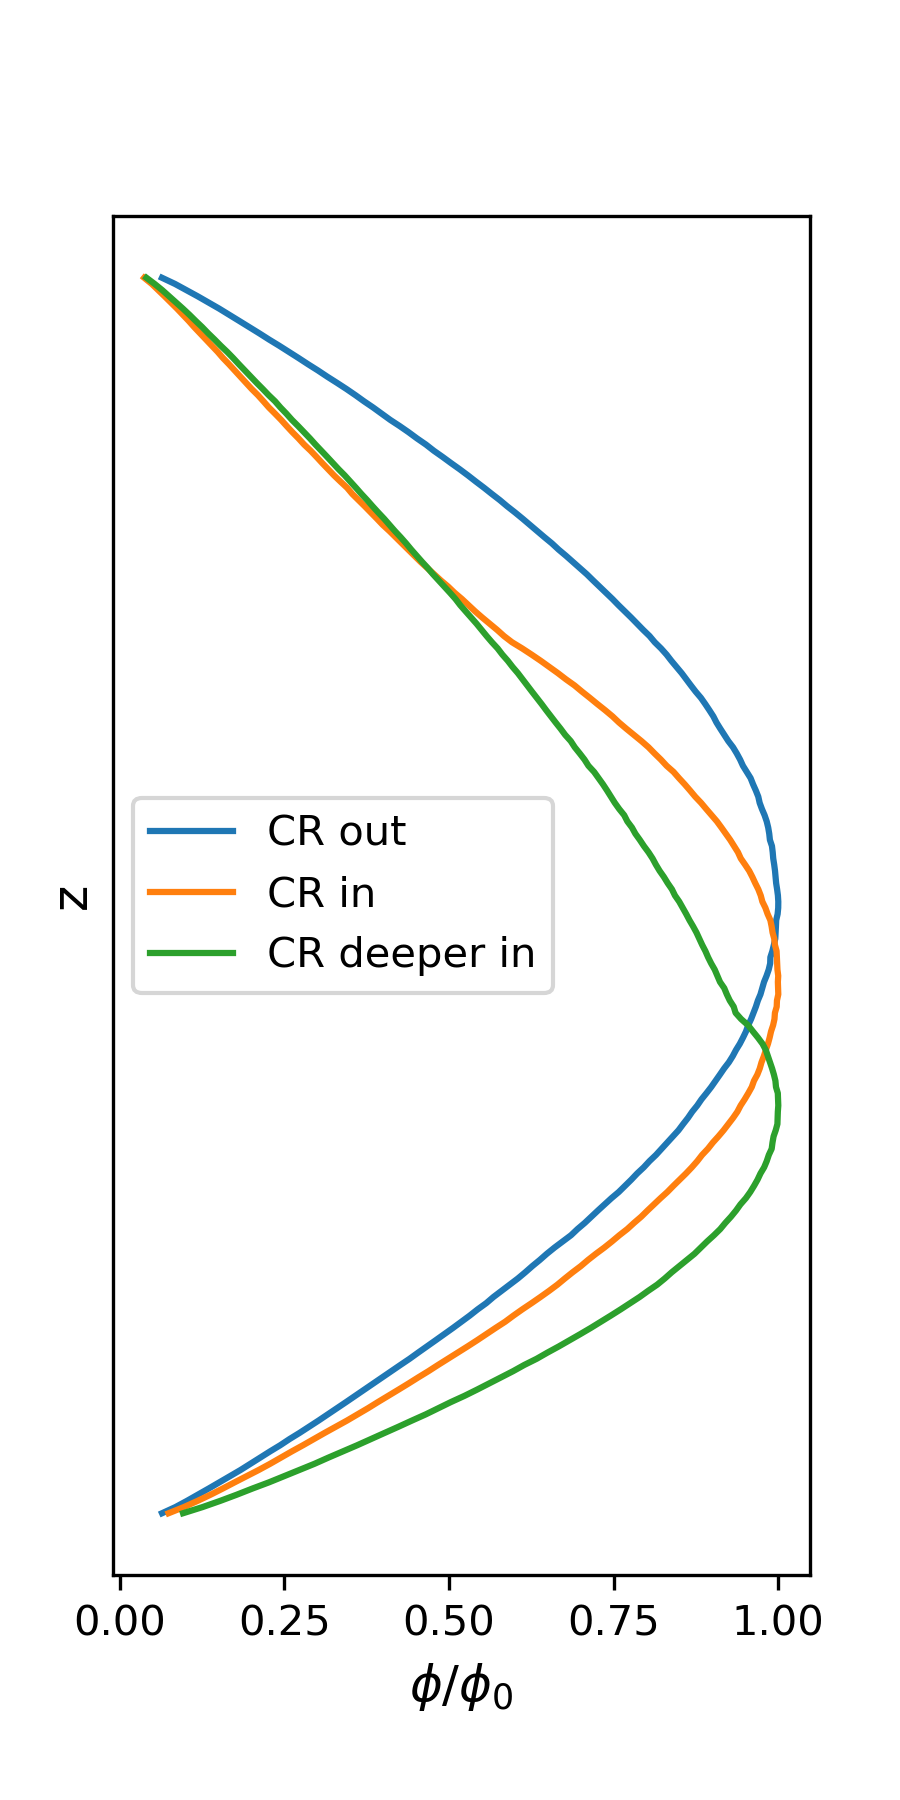
\includegraphics[scale=0.46] {figures/04-controlrod.png}}\protect
\caption{\label{fig:controlrod} \footnotesize{Change in the axial flux shape due to control rod insertion.}}
\end{figure}

\subsection{Control rods}

It is noteworthy to mention that certain elements in the reactor, such as control rods, can drastically change the spatial distribution of neutrons in the core, and also have an impact on the multiplication factor of the system. Figure \ref{fig:controlrod} illustrates the influence of a control rod insertion on the axial flux. We can see that the peak of the flux will shift to deeper regions of the core. The impact of the rod on the reactivity 

\[
\rho=\frac{k-1}{k}
\]

\noindent can be given by the control rod worth, which describes the change in the k-effective $\Delta k$ due to the insertion of the control rod.  

\subsection{Calculation scheme}

As a final note to our discussion on neutron transport, it is important to highlight that in this chapter we have barely scratched the surface. There is no numerical solution to the transport problem which can be applied directly at each levels of the reactor core besides Monte Carlo methods. Therefore the problem is typically split into tasks as illustrated with an oversimplified scheme in Figure \ref{fig:calculationscheme}. First the continuous cross section data is processed to obtain group-wise data. Then this is used to tackle the slowing down and thermalization problem at a pin or lattice level to obtain few group cross sections. Finally that is used in core level diffusion solvers. There can be of course other task to include depending the application, such as depletion calculations, or transient calculations, which are the topics of the following chapters.

\begin{figure}[ht!]
\protect \centering{
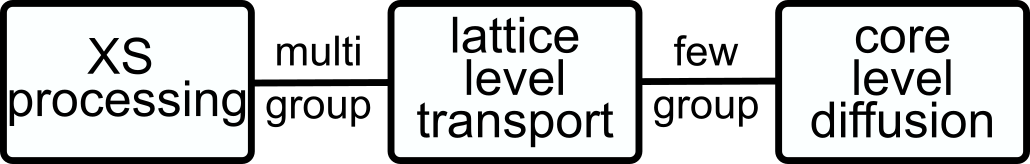
\includegraphics[scale=0.46] {figures/calculationscheme.png}}\protect
\caption{\label{fig:calculationscheme} \footnotesize{Schematic illustration of the reactor calculation process.}}
\end{figure} 


%\end{document}
